\documentclass[compress,mathserif]{beamer}
\usepackage{beamerthemesplit_z}
\usepackage{bm,bbm,graphicx}
\usepackage[czech]{babel}
\usepackage{pgf,pgfarrows,pgfnodes,pgfautomata,pgfheaps}
\usepackage{yhmath,amsmath,amssymb,amsbsy}
\usepackage[utf8]{inputenc}
\usepackage[style=german]{csquotes}


\title[Popisná statistika]{Popisná statistika}
\author{Lenka Křivánková}
\institute{142474@mail.muni.cz}
\date{}

\usetemplatetocsection
%{\color{structure}\inserttocsection}
{\color{structure}\insertsection}


\begin{document}
\shorthandoff{-} %opravuje chybu czech babel
\frame{\titlepage
\begin{center}

	{Přednáška Statistika 1 (BKMSTA1)\\[5mm] 8. říjen 2016, Brno}
\end{center}}%\rule[-1.9cm]{5cm}{0cm}



\frame {
  \frametitle{Motivace}
  \begin{itemize}
\item Popisná statistika slouží zejména k prezentaci dat a výsledků. 

\item Číselné charakteristiky informují o úrovni, variabilitě a těsnosti závislosti znaků.

\item V dalším budeme probírat analogické veličiny u náhodných výběrů.

\end{itemize}
}

\frame{
\centerline{\bf Základní, výběrový a datový soubor}
}


\frame {
  \frametitle{Základní a výběrový soubor}
\begin{itemize}
\item {\bf Základním souborem} rozumíme libovolnou neprázdnou množinu $E$. Její prvky
značíme $\epsilon$ a nazýváme je objekty. 

\item Libovolnou neprázdnou podmnožinu $\{\epsilon_1,\dots , \epsilon_n\}$ základního souboru $E$ nazýváme {\bf výběrový soubor} rozsahu $n$.

\item Je-li $G \subseteq E$, pak symbolem $N(G)$ rozumíme {\bf absolutní četnost} množiny $G$
ve výběrovém souboru, tj. počet těch objektů množiny $G$, které patří do
výběrového souboru. 

\item {\bf Relativní četnost} množiny $G$ ve výběrovém souboru zavedeme
vztahem
$$p(G) =\frac{N(G)}{n}.$$
\end{itemize}
}

\frame {
  \frametitle{Základní a výběrový soubor -- příklad}
  Hodnocení finančního zdraví několika firem dvěma hodnotiteli.
  \begin{center}
\begin{tabular}{cc}
I. hodnotitel&II. hodnotitel\\ \hline
2& 2 \\
1& 3 \\
4 &3 \\
1 &1 \\
1 &2 \\
4 &4 \\
3 &3 \\
3& 4 \\
1 &1 \\
1& 1 \\
\end{tabular}
\begin{tabular}{cc}
I. hodnotitel&II. hodnotitel\\ \hline
4& 2 \\
4& 4 \\
2& 2 \\
4& 3 \\
2& 3 \\
4& 4 \\
1 &1 \\
4 &3 \\
4 &4 \\
1 &3 \\
\end{tabular}
\end{center}
Hodnocení I. hodnotitele budeme dále označovat $X$ a hodnocení II. hodnotitele $Y$.
}





\frame {
  \frametitle{Datový soubor}
Nechť je dán výběrový soubor $ \{ \epsilon_1, \dots , \epsilon_n \} \subseteq E$. Hodnoty znaků $X,Y, Z$ pro $i$-tý objekt označíme $x_i = X(\epsilon_i)$, $y_i = Y(\epsilon_i)$, $\dots$, $z_i = Z(\epsilon_i)$, $i = 1, \dots , n$.\\[0.5cm]

Matice
$$\left[
\begin{array}{cccc}
x_1& y_1& \cdots &z_1\\
x_2& y_2& \cdots &z_2\\
\vdots&\vdots&&\vdots\\
x_n& y_n& \cdots &z_n\\
\end{array}\right]
$$
typu $n \times p$ se nazývá {\bf datový soubor}. Její řádky odpovídají jednotlivým objektům, sloupce znakům.
Libovolný sloupec této matice nazýváme jednorozměrným datovým souborem.
}




\frame {
  \frametitle{Datový soubor}
Jestliže uspořádáme hodnoty některého znaku (např. znaku $X$) v jednorozměrném datovém souboru vzestupně podle velikosti, dostaneme {\bf uspořádaný datový soubor}
$$\left[
\begin{array}{c}
x_{(1)}\\
\vdots\\
x_{(n)}\\
\end{array}\right]
,
$$
kde $x_{(1)} \leq x_{(2)} \leq \cdots \leq x_{(n)}$.\\[0.2cm] 
Vektor
$$\left[
\begin{array}{c}
x_{[1]}\\
\vdots\\
x_{[r]}\\
\end{array}\right]
,
$$
kde $x_{[1]} < \cdots < x_{[r]}$ jsou navzájem různé hodnoty znaku $X$, se nazývá {\bf vektor
variant}.
}

\frame {
  \frametitle{Datový soubor -- příklad}
  \scriptsize
$$\left[\begin{array}{c}
2\\
1\\
4\\
1\\
1\\
4\\
3\\
3\\
1\\
1\\
4\\
4\\
2\\
4\\
2\\
4\\
1\\
4\\
4\\
1\\
\end{array}\right]
,
\left[\begin{array}{c}
1\\
1\\
1\\
1\\
1\\
1\\
1\\
2\\
2\\
2\\
3\\
3\\
4\\
4\\
4\\
4\\
4\\
4\\
4\\
4\\
\end{array}\right]
, 
\left[\begin{array}{c}
1\\
2\\
3\\
4\\
\end{array}\right]
  $$
  \normalsize
}


\frame{
\centerline{\bf Bodové rozdělení četností}
}

\frame {
  \frametitle{Bodové rozdělení četnosti}

Nechť je dán jednorozměrný datový soubor. Jestliže počet variant znaku $X$
není příliš velký, pak přiřazujeme četnosti jednotlivým variantám a hovoříme
o {\bf bodovém rozdělení četností}.
}



\frame {
  \frametitle{Bodové rozdělení četnosti}
Existuje několik způsobů, jak graficky znázornit bodové rozdělení četností.
\begin{itemize}
\item {\bf Tečkový diagram}: na číselné ose vyznačíme jednotlivé varianty znaku $X$ a
nad každou variantu nakreslíme tolik teček, jaká je její absolutní četnost.
\item {\bf Polygon četnosti}: je lomená čára spojující body, jejichž $x$-ová souřadnice je
varianta znaku $X$ a $y$-ová souřadnice je absolutní četnost této varianty.
\end{itemize}
}



\frame {
  \frametitle{Bodové rozdělení četnosti}
  \begin{itemize}
\item {\bf Sloupkový diagram}: je soustava na sebe nenavazujících obdélníků, kde střed
základny je varianta znaku $X$ a výška je absolutní četnost této varianty.
\item {\bf Výsečový graf}: je kruh rozdělený na výseče, jejichž vnější obvod odpovídá
absolutním četnostem variant znaku $X$.
\item {\bf Dvourozměrný tečkový diagram}: na vodorovnou osu vyneseme varianty znaku
$X$, na svislou varianty znaku $Y$ a do příslušných průsečíků nakreslíme tolik
teček, jaká je absolutní četnost dané dvojice.
\end{itemize}
}



\frame {
  \frametitle{Bodové rozdělení četnosti -- příklad}
  \vspace*{0cm}
Pro datový soubor "hodnocení finančního zdraví několika firem" sestrojte\\[0.5cm]
\begin{overprint}
\onslide<1>
\begin{center}jednorozměrné tečkové diagramy pro znak $X$ a znak $Y$\\[1cm]
\scalebox{0.5}{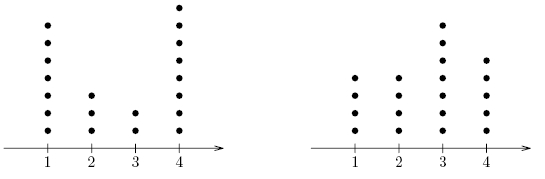
\includegraphics{b1.jpg}}\end{center}
\onslide<2>
\begin{center}polygony četností pro znak $X$ a znak $Y$\\[1cm]
\scalebox{0.5}{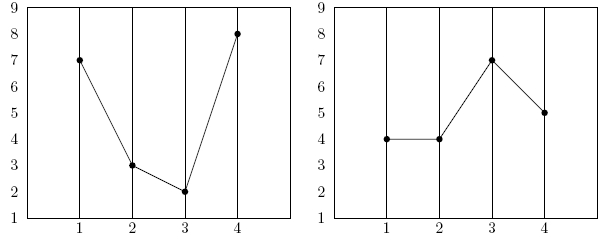
\includegraphics{b2.jpg}} \end{center}
\onslide<3>
\begin{center}sloupkové diagramy pro znak $X$ a znak $Y$\\[1cm]
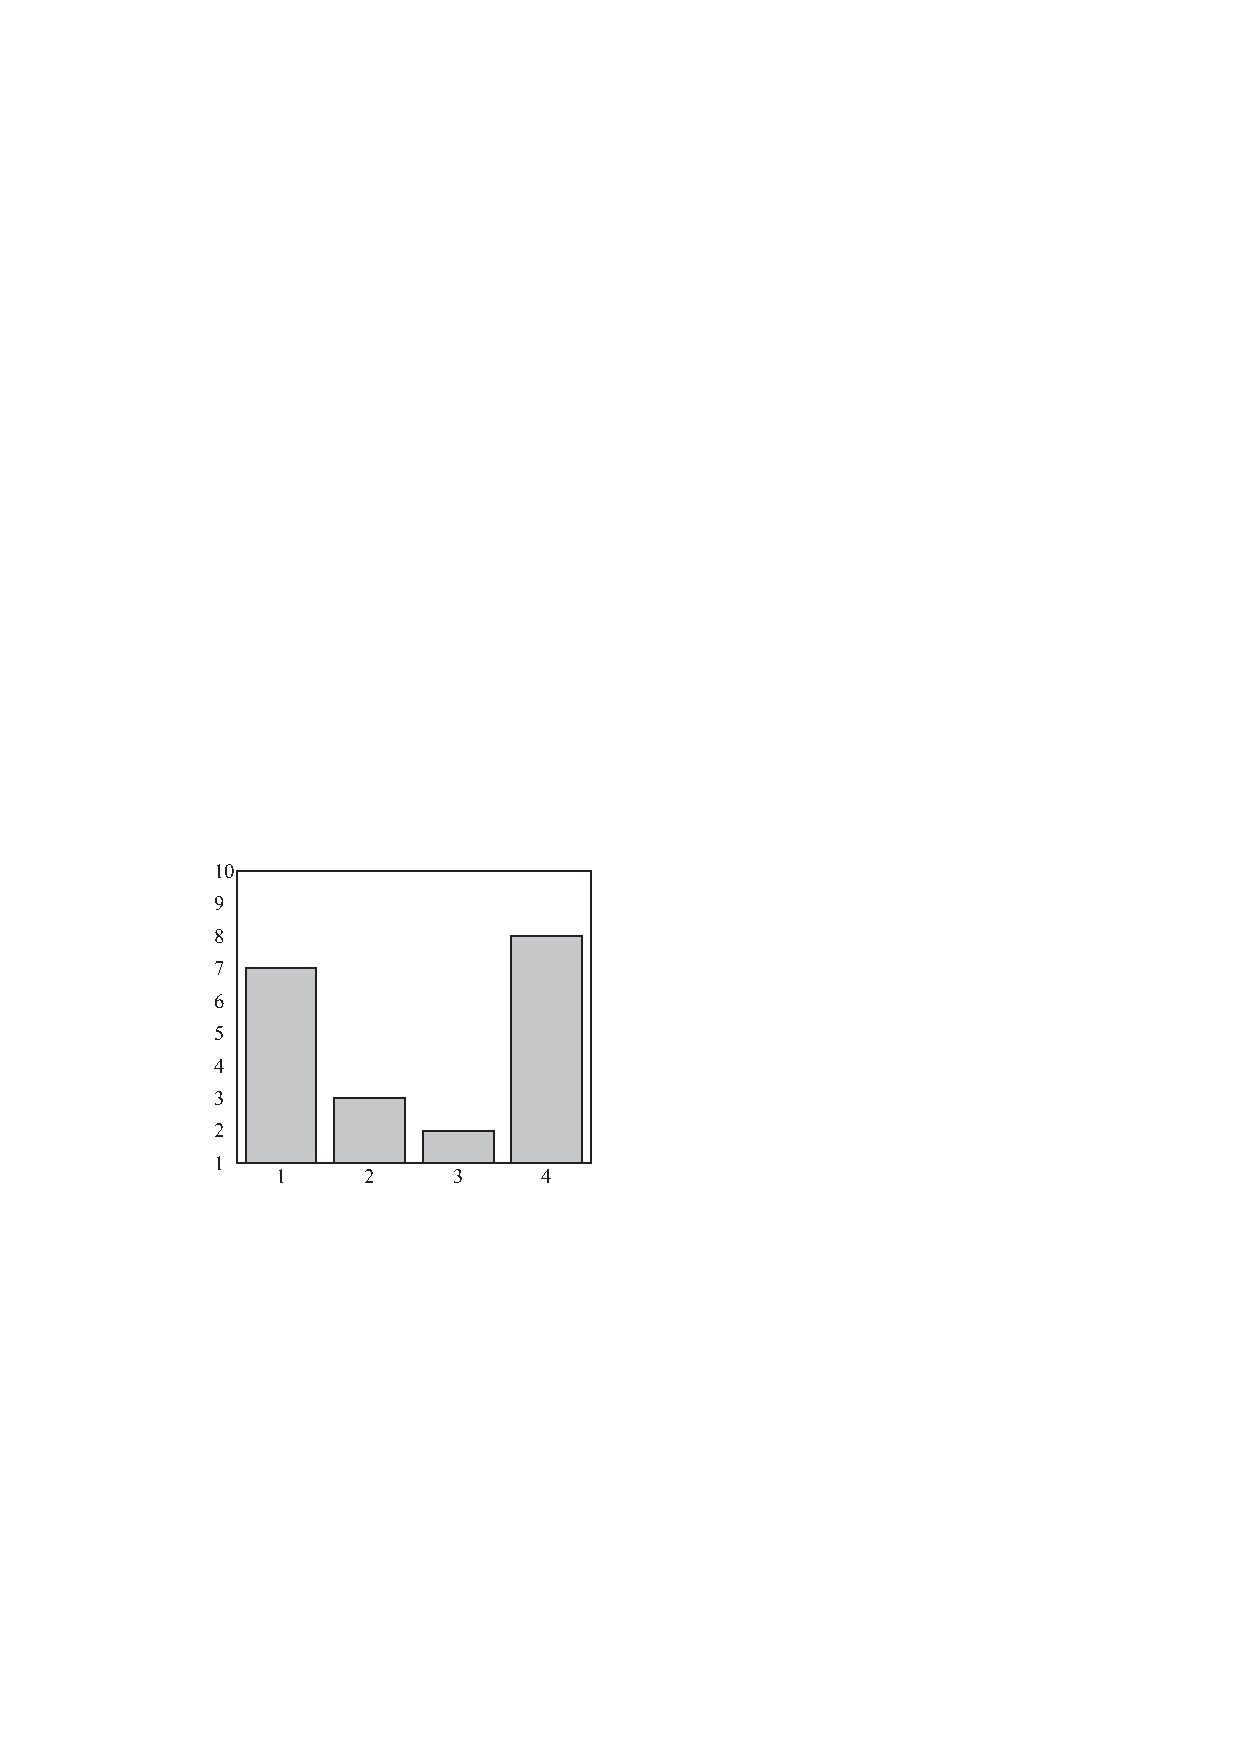
\includegraphics[width=5.1cm]{obr2-5new.pdf}\quad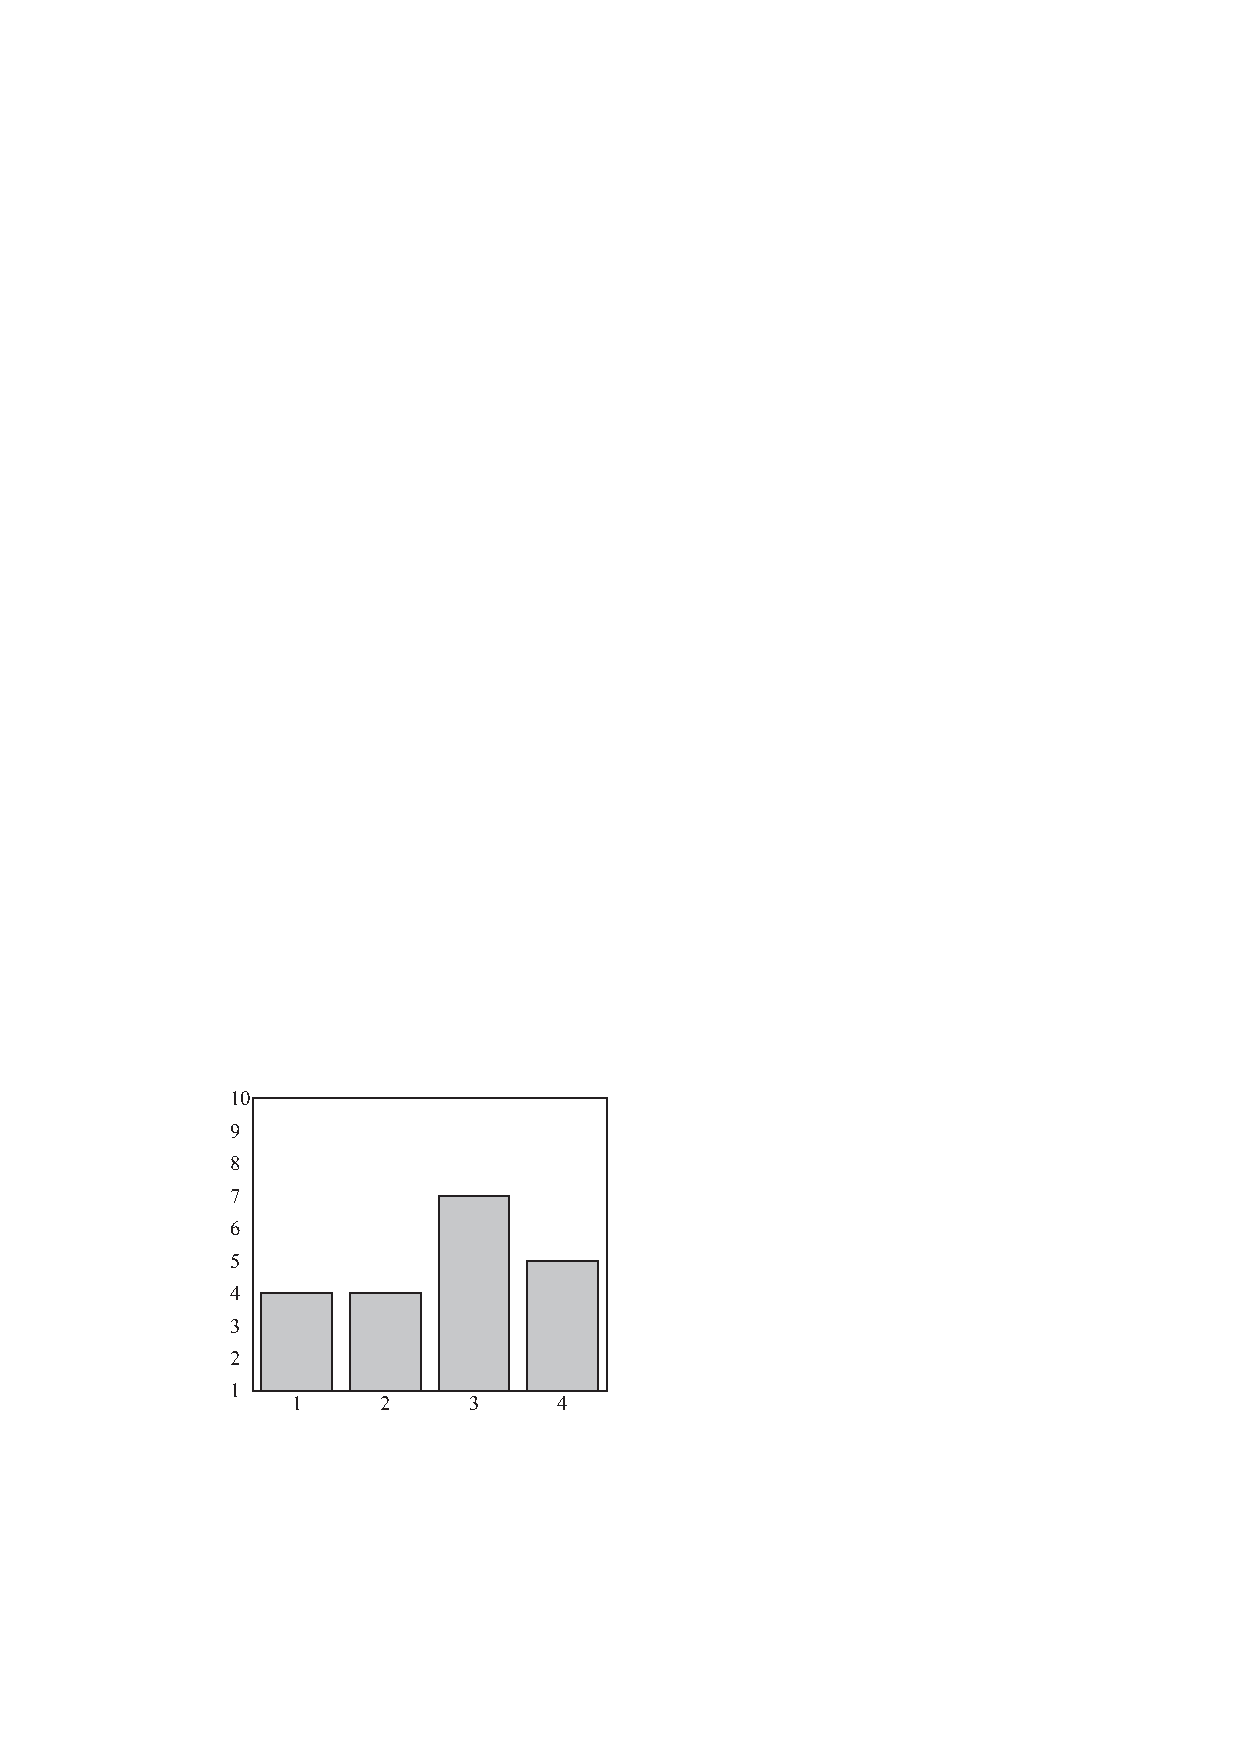
\includegraphics[width=5.1cm]{obr2-6new.pdf} 
\end{center}
\onslide<4>
\begin{center}výsečové diagramy pro znak $X$ a znak $Y$\\[1cm]
\scalebox{0.5}{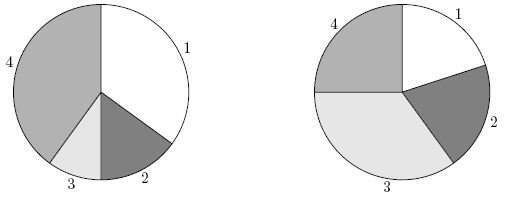
\includegraphics{b4.jpg}} \end{center}
\onslide<5>
\begin{center} dvourozměrný tečkový diagram pro vektorový znak $(X, Y)$\\[0.5cm]
\scalebox{0.5}{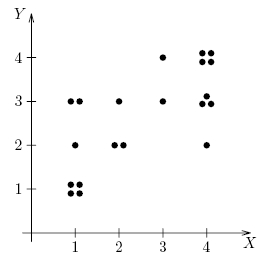
\includegraphics{b5.jpg}}\end{center}

\end{overprint}
}







\frame {
  \frametitle{Variační řada}
  \begin{itemize}
  \item
Bodové rozdělení četností lze znázornit nejenom graficky, ale též tabulkou
zvanou {\bf variační řada}, která obsahuje absolutní a relativní četnosti jednotlivých variant znaku v daném výběrovém souboru a též absolutní a relativní
kumulativní četnosti. \\[0.5cm]
\item
Pomocí relativních četností se zavádí četnostní funkce,
pomocí relativních kumulativních četností empirická distribuční funkce (je
pro ni typické, že má schodovitý průběh). 
\end{itemize}

}

\frame {
  \frametitle{Variační řada}

Nechť je dán jednorozměrný datový soubor, v němž znak $X$ nabývá $r$ variant.
Pro $j = 1, \dots , r$ definujeme:
\begin{itemize}
\item {\bf absolutní četnost} varianty $x_{[j]}$ ve výběrovém souboru
$$n_j = N(X = x_{[j]})$$
\item {\bf relativní četnost} varianty $x_{[j]}$ ve výběrovém souboru
$$p_j =\frac{n_j}{n}$$
\item {\bf absolutní kumulativní četnost} prvních $j$ variant ve výběrovém souboru
$$N_j = N(X \leq x_{[j]}) = n_1 + \dots + n_j$$
\item {\bf relativní kumulativní četnost} prvních $j$ variant ve výběrovém souboru
$$F_j =\frac{N_j}{n}= p_1 + \dots + p_j$$
\end{itemize}

}

\frame {
  \frametitle{Variační řada}

Tabulka typu
\begin{center}
\begin{tabular}{|c||c|c|c|c|}
\hline
$x_{[j]}$& $n_j$& $p_j$& $N_j$& $F_j$\\ \hline \hline
$x_{[1]}$& $n_1$ &$p_1$& $N_1$& $F_1$\\ \hline
$\vdots$&
$\vdots$&
$\vdots$&
$\vdots$&
$\vdots$\\ \hline
$x_{[r]}$& $n_r$& $p_r$& $N_r$ &$F_r$\\ \hline
\end{tabular}
\end{center}
se nazývá {\bf variační řada}.
}



\frame {
  \frametitle{Variační řada -- příklad}
Pro datový soubor "hodnocení finančního zdraví několika firem" sestavte variační řadu pro znak $X$. 
\begin{center}
%\scalebox{0.5}{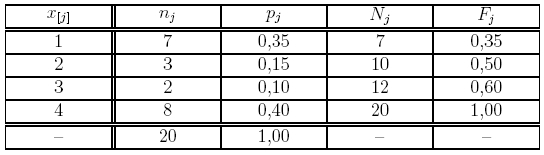
\includegraphics{b6.jpg}} 
\begin{tabular}{|c||c|c|c|c|}
\hline
\parbox{1.5cm}{\mbox{}\hfill$x_{[j]}$\hfill\mbox{}} & \parbox{1.5cm}{\mbox{}\hfill$n_j$\hfill\mbox{}} & \parbox{1.5cm}{\mbox{}\hfill$p_j$\hfill\mbox{}} & \parbox{1.5cm}{\mbox{}\hfill$N_j$\hfill\mbox{}} & \parbox{1.5cm}{\mbox{}\hfill$F_j$\hfill\mbox{}} \\
\hline
\hline
1	& 7 &	0,35 & 7 & 0,35 \\
\hline
2	& 3	& 0,15 & 10 & 0,50 \\
\hline
3	& 2	& 0,10 & 12 & 0,60 \\
\hline
4	& 8	& 0,40 & 20 & 1,00 \\
\hline\hline
--	& 20 & 1,00 & -- & -- \\
\hline\end{tabular}
\end{center}

}

\frame {
  \frametitle{Četnostní a empirická distribuční funkce}
Funkce
$$
p(x) = \left\{ \begin{array}{cl}
p_j &\mathsf{pro}\quad x = x_{[j]},\quad j = 1, \dots , r\\
0 &\mathsf{jinak}
\end{array}\right.
$$
se nazývá {\bf četnostní funkce}.\\[0.5cm] 

Funkce
$$
F(x) =\left\{\begin{array}{cl}
0 &\mathsf{pro}\quad x < x_{[1]}\\
F_j& \mathsf{pro}\quad x_{[j]} \leq x < x_{[j+1]},\quad j = 1, \dots , r - 1\\
1 &\mathsf{pro}\quad x \geq x_{[r]}\\
\end{array}\right.
$$
se nazývá {\bf empirická distribuční funkce}.
}



\frame {
  \frametitle{Četnostní a empirická distribuční funkce -- příklad}
\begin{center}
\vspace{-0.3cm}
\begin{tabular}{cc}
\begin{tabular}{c}
\scalebox{0.49}{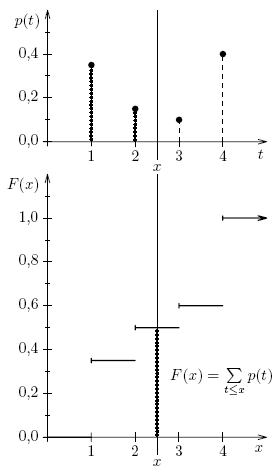
\includegraphics{b7.jpg}}\\
\end{tabular}
&
 \begin{tabular}{p{4cm}}
Pro datový soubor "hodnocení finančního zdraví několika firem" nakreslete
grafy četnostní funkce a empirické distribuční funkce znaku $X$.
\end{tabular}
\end{tabular}

\end{center}
}



\frame {
  \frametitle{Četnostní a empirická distribuční funkce -- vlastnosti}
\begin{itemize}
\item Četnostní funkce je 
\begin{itemize}
\item nezáporná ($\forall x \in R: p(x) \geq 0$) a
\item normovaná, tj.
$$
\sum_{x=-\infty}^\infty p(x) = 1.
$$
\end{itemize}
\item Empirická distribuční funkce je 
\begin{itemize}
\item neklesající, tzn.
$$\forall x_1, x_2 \in R, x_1 < x_2 : F(x_1) \leq F(x_2),$$
\item zprava spojitá ($\forall x_0 \in R$ libovolné, ale pevně dané: $\lim_{x \rightarrow x_0}
F(x) = F(x_0)$) a 
\item normovaná ($\lim_{x \rightarrow - \infty}F(x) = 0$, $\lim_{x \rightarrow  \infty}F(x) = 1$).
\end{itemize}
\end{itemize}
}


\frame {
  \frametitle{Dvourozměrný datový soubor}
Nechť je dán dvourozměrný datový soubor
$$
\left[
\begin{array}{cc}
x_1& y_1\\
\vdots&\vdots\\
x_n &y_n\\
\end{array}\right]
,
$$
kde znak $X$ má $r$ variant a znak $Y$ má $s$ variant. Pak definujeme:
\begin{itemize}
\item {\bf simultánní absolutní četnost} dvojice $(x_{[j]}, y_{[k]})$ ve výběrovém souboru
$$n_{jk} = N(X = x_{[j]} \wedge Y = y_{[k]}),$$
\item {\bf simultánní relativní četnost} dvojice $(x_{[j]}, y_{[k]})$ ve výběrovém souboru
$$
p_{jk} =\frac{n_{jk}}{n},
$$
\end{itemize}
}


\frame {
  \frametitle{Dvourozměrný datový soubor}
  \begin{itemize}
  
\item {\bf marginální absolutní četnost} varianty $x_{[j]}$
$$
n_{j.} = N(X = x_{[j]}) = n_{j1} + \dots + n_{js},
$$
\item {\bf marginální relativní četnost} varianty $x_{[j]}$
$$
p_{j.} =\frac{n_{j.}}{n}= p_{j1} + \dots + p_{js},
$$

\item {\bf marginální absolutní četnost} varianty $y_{[k]}$
$$
n_{.k} = N(Y = y_{[k]}) = n_{1k} + \dots + n_{rk},
$$
\item {\bf marginální relativní četnost} varianty $y_{[k]}$
$$
p_{.k} =\frac{n_{.k}}{n}= p_{1k} + \dots + p_{rk},
$$
\end{itemize}
}


\frame {
  \frametitle{Dvourozměrný datový soubor}
  \begin{itemize}
\item {\bf sloupcově podmíněná relativní četnost} varianty $x_{[j]}$ za předpokladu $y_{[k]}$
$$
p_{j(k)} =\frac{n_{jk}}{n_{.k}},
$$
\item {\bf řádkově podmíněná relativní četnost} varianty $y_{[k]}$ za předpokladu $x_{[j]}$
$$
p_{(j)k} =\frac{n_{jk}}{n_{j.}}.
$$
\end{itemize}
}


\frame {
  \frametitle{Dvourozměrný datový soubor}
Kteroukoliv ze simultánních četností či podmíněných relativních četností zapisujeme
do kontingenční tabulky. {\bf Kontingenční tabulka} simultánních absolutních četností má tvar
\begin{center}
%\scalebox{0.5}{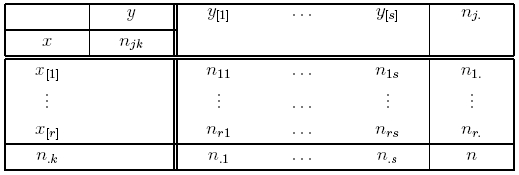
\includegraphics{b8.jpg}} 
\begin{tabular}{|cc||ccc|c|}
\hline
\multicolumn{1}{|c|}{\parbox{1.2cm}{\mbox{}}}& \parbox{1.2cm}{\mbox{}\hfill$y$\hfill\mbox{}} & \parbox{1.2cm}{\mbox{}\hfill$y_{[1]}$\hfill\mbox{}} & \parbox{1.2cm}{\mbox{}\hfill$\dots$\hfill\mbox{}} & \parbox{1.2cm}{\mbox{}\hfill$y_{[s]}$\hfill\mbox{}} & \parbox{1.2cm}{\mbox{}\hfill$n_{j.}$\hfill\mbox{}} \\[.75mm]
\cline{1-2}
\multicolumn{1}{|c|}{$x$} & $n_{jk}$ & & & & \\[.75mm]
\hline\hline
$x_{[1]}$ & & $n_{11}$ & $\dots$ & $n_{1s}$ & $n_{1.}$ \\[.75mm]
$\vdots$ & & $\vdots$ & $\dots$ & $\vdots$ & $\vdots$ \\[.75mm]
$x_{[r]}$ & & $n_{r1}$ & $\dots$ & $n_{rs}$ & $n_{r.}$ \\[.75mm]
\hline
$n_{.k}$ & & $n_{.1}$ & $\dots$ & $n_{.s}$ & $n$ \\[.75mm]
\hline
\end{tabular}
\end{center}
}

\frame {
  \frametitle{Simultánní četnostní funkce}
Funkce
$$
p(x, y) = \left\{\begin{array}{ll}
p_{jk}& \mathsf{pro}\quad x = x_{[j]}, y = y_{[k]},\quad j = 1, \dots, r,\quad k = 1, \dots, s\\
0& \mathsf{jinak}
\end{array}\right.
$$
se nazývá {\bf simultánní četnostní funkce}. Četnostní funkce pro znaky $X$ a $Y$
(tzv. {\bf marginání četnostní funkce}) odlišíme indexem takto:
$$
p_1(x) = \left\{ 
\begin{array}{ll}
p_{j.}& \mathsf{pro}\quad x = x_{[j]},\quad j = 1, \dots, r\\
0 &\mathsf{jinak}\\
\end{array}\right.
$$
$$
p_2(y) = \left\{ 
\begin{array}{ll}
p_{.k}& \mathsf{pro}\quad y = y_{[k]},\quad k = 1, \dots, s\\
0 &\mathsf{jinak}\\
\end{array}
\right.
$$
}



\frame{
\frametitle{Podmíněné četnostní funkce}


Funkce $p_{1\left|2\right.} \left(x\left|y\right. \right)$ zavedená vztahem $\forall x\in \mathbb R$:
$$
p_{1\left|2\right. } \left(x\left|y\right. \right)=\left\{
\begin{array}{ll} 
\frac{p\left(x,y\right)}{p_{2} \left(y\right)} &\mathrm{pro\; }p_{2} \left(y\right)>0 \\ 
0 &\mathrm{jinak} 
\end{array}\right. 
$$ 
se nazývá \textbf{sloupcově podmíněná četnostní funkce.}\\[5mm]

Funkce $p_{2\left|1\right. } \left(y\left|x\right. \right)$ zavedená vztahem $\forall y\in \mathbb R$:
$$
p_{2\left|1\right. } \left(y\left|x\right. \right)=\left\{
\begin{array}{ll} 
\frac{p\left(x,y\right)}{p_{1} \left(x\right)} & \mathrm{pro\; }p_{1} \left(x\right)>0 \\ 
0& \mathrm{jinak} 
\end{array}\right. 
$$ 
se nazývá \textbf{řádkově podmíněná četnostní funkce.}
}


\frame {
  \frametitle{Četnostní nezávislost}
Znaky $X$, $Y$ jsou v~daném výběrovém souboru \textbf{četnostně nezávislé}, jestliže platí: 
$$
\forall j=1, \dots, r,\ \forall k=1, \dots, s:\quad p_{jk}=p_{j.}\cdot p_{.k}
$$ 
neboli
$$
\forall (x,y)\in\mathbb R^2:\ p(x,y)=p_1(x)\cdot p_2(y).
$$
}


\frame {
  \frametitle{Četnostní nezávislost -- ekvivalentní definice}
Znaky $X$, $Y$ jsou v~daném výběrovém souboru \textbf{četnostně nezávislé}, jestliže platí: 
$$
\forall y\in \mathbb R,\ p_{2} \left(y\right)>0:\quad p_{1\left|2\right. } \left(x\left|y\right. \right)=p_{1} \left(x\right)
$$ 
resp. 
$$
\forall x\in \mathbb R,\ p_{1} \left(x\right)>0:\quad p_{2\left|1\right. } \left(y\left|x\right. \right)=p_{2} \left(y\right).
$$
}


\frame {
  \frametitle{Dvourozměrný datový soubor -- příklad}
  
Pro datový soubor "hodnocení finančního zdraví několika firem"\\[0.5cm]
\begin{overprint}
\onslide<1>
$\bullet$ sestavte kontingenční tabulku simultánních absolutních četností

\begin{center}

%\scalebox{0.5}{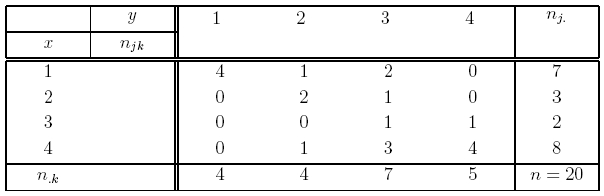
\includegraphics{b9.jpg}} 

\begin{tabular}{|cc||cccc|c|}
\hline
\multicolumn{1}{|c|}{\parbox{1.0cm}{\mbox{}}}& \parbox{1.0cm}{\mbox{}\hfill$y$\hfill\mbox{}} & \parbox{1.0cm}{\mbox{}\hfill 1 \hfill\mbox{}} & \parbox{1.0cm}{\mbox{}\hfill 2 \hfill\mbox{}} & \parbox{1.0cm}{\mbox{}\hfill 3 \hfill\mbox{}} & \parbox{1.0cm}{\mbox{}\hfill 4 \hfill\mbox{}} & \parbox{1.0cm}{\mbox{}\hfill$n_{j.}$\hfill\mbox{}} \\[.75mm]
\cline{1-2}
\multicolumn{1}{|c|}{$x$} & $n_{jk}$ & & & & & \\[.75mm]
\hline\hline
1 & & 4 & 1 & 2 & 0 & 7 \\[.75mm]
2 & & 0 & 2 & 1 & 0 & 3 \\[.75mm]
3 & & 0 & 0 & 1 & 1 & 2 \\[.75mm]
4 & & 0 & 1 & 3 & 4 & 8 \\[.75mm]
\hline
$n_{.k}$ & & 4 & 4 & 7 & 5 & $n=20$ \\[.75mm]
\hline
\end{tabular}\end{center}

\onslide<2>
$\bullet$ sestavte kontingenční tabulku simultánních relativních četností

\begin{center}

%\scalebox{0.5}{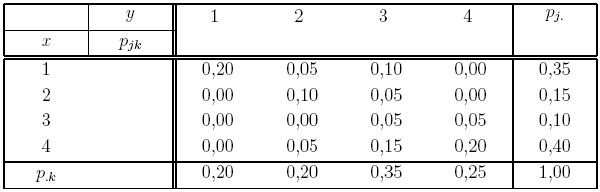
\includegraphics{b10.jpg}} 

\begin{tabular}{|cc||cccc|c|}
\hline
\multicolumn{1}{|c|}{\parbox{1.0cm}{\mbox{}}}& \parbox{1.0cm}{\mbox{}\hfill$y$\hfill\mbox{}} & \parbox{1.0cm}{\mbox{}\hfill 1 \hfill\mbox{}} & \parbox{1.0cm}{\mbox{}\hfill 2 \hfill\mbox{}} & \parbox{1.0cm}{\mbox{}\hfill 3 \hfill\mbox{}} & \parbox{1.0cm}{\mbox{}\hfill 4 \hfill\mbox{}} & \parbox{1.0cm}{\mbox{}\hfill$p_{j.}$\hfill\mbox{}} \\[.75mm]
\cline{1-2}
\multicolumn{1}{|c|}{$x$} & $p_{jk}$ & & & & & \\[.75mm]
\hline\hline
1 & & 0,20 & 0,05 & 0,10 & 0,00 & 0,35 \\[.75mm]
2 & & 0,00 & 0,10 & 0,05 & 0,00 & 0,15 \\[.75mm]
3 & & 0,00 & 0,00 & 0,05 & 0,05 & 0,10 \\[.75mm]
4 & & 0,00 & 0,05 & 0,15 & 0,20 & 0,40 \\[.75mm]
\hline
$p_{.k}$ & & 0,20 & 0,20 & 0,35 & 0,25 & 1,00 \\[.75mm]
\hline
\end{tabular}

\end{center}

\onslide<3>
$\bullet$ nakreslete graf simultánní četnostní funkce $p(x, y)$
\begin{center}\scalebox{0.5}{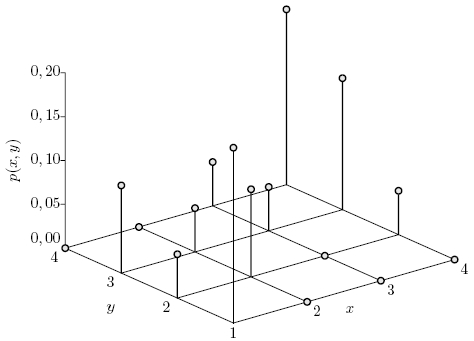
\includegraphics{b11.jpg}} \end{center}

\onslide<4> $\bullet$ sestavte kontingenční tabulku sloupcově  podmíněných relativních četností
\begin{center}
%\scalebox{0.5}{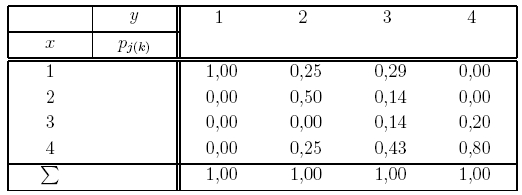
\includegraphics{b12.jpg}} 

\begin{tabular}{|cc||cccc|}
\hline
\multicolumn{1}{|c|}{\parbox{1.0cm}{\mbox{}}}& \parbox{1.0cm}{\mbox{}\hfill$y$\hfill\mbox{}} & \parbox{1.0cm}{\mbox{}\hfill 1 \hfill\mbox{}} & \parbox{1.0cm}{\mbox{}\hfill 2 \hfill\mbox{}} & \parbox{1.0cm}{\mbox{}\hfill 3 \hfill\mbox{}} & \parbox{1.0cm}{\mbox{}\hfill 4 \hfill\mbox{}}  \\[.75mm]
\cline{1-2}
\multicolumn{1}{|c|}{$x$} & $p_{j(k)}$ & & & &  \\[.75mm]
\hline\hline
1 & & 1,00 & 0,25 & 0,29 & 0,00 \\[.75mm]
2 & & 0,00 & 0,50 & 0,14 & 0,00 \\[.75mm]
3 & & 0,00 & 0,00 & 0,14 & 0,20 \\[.75mm]
4 & & 0,00 & 0,25 & 0,43 & 0,80 \\[.75mm]
\hline
$\sum$ & & 1,00 & 1,00 & 1,00 & 1,00 \\[.75mm]
\hline
\end{tabular}


\end{center}

\onslide<5> $\bullet$ sestavte kontingenční tabulku řádkově podmíněných relativních četností
\begin{center}


%\scalebox{0.5}{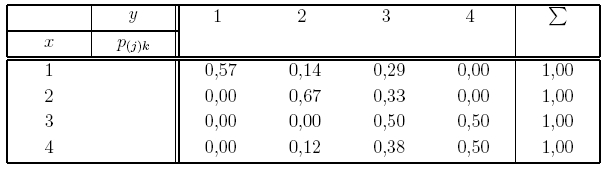
\includegraphics{b13.jpg}} 

\begin{tabular}{|cc||cccc|c|}
\hline
\multicolumn{1}{|c|}{\parbox{1.0cm}{\mbox{}}}& \parbox{1.0cm}{\mbox{}\hfill$y$\hfill\mbox{}} & \parbox{1.0cm}{\mbox{}\hfill 1 \hfill\mbox{}} & \parbox{1.0cm}{\mbox{}\hfill 2 \hfill\mbox{}} & \parbox{1.0cm}{\mbox{}\hfill 3 \hfill\mbox{}} & \parbox{1.0cm}{\mbox{}\hfill 4 \hfill\mbox{}} & \parbox{1.0cm}{\mbox{}\hfill$\sum$\hfill\mbox{}} \\[.75mm]
\cline{1-2}
\multicolumn{1}{|c|}{$x$} & $p_{(j)k}$ & & & & & \\[.75mm]
\hline\hline
1 & & 0,57 & 0,14 & 0,29 & 0,00 & 1,00 \\[.75mm]
2 & & 0,00 & 0,67 & 0,33 & 0,00 & 1,00 \\[.75mm]
3 & & 0,00 & 0,00 & 0,50 & 0,50 & 1,00 \\[.75mm]
4 & & 0,00 & 0,12 & 0,38 & 0,50 & 1,00 \\[.75mm]
\hline
\end{tabular}

\end{center}

\onslide<6> $\bullet$  zjistěte, kolik procent firem, kterým první hodnotitel udělil jedničku, mělo od druhého hodnotitele dvojku
\begin{center}

%\scalebox{0.5}{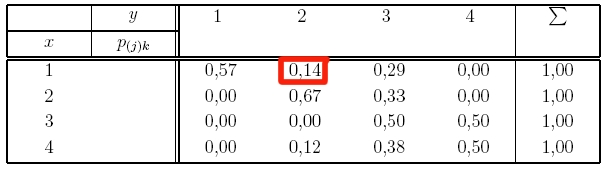
\includegraphics{b14.jpg}} 

\begin{tabular}{|cc||cccc|c|}
\hline
\multicolumn{1}{|c|}{\parbox{1.0cm}{\mbox{}}}& \parbox{1.0cm}{\mbox{}\hfill$y$\hfill\mbox{}} & \parbox{1.0cm}{\mbox{}\hfill 1 \hfill\mbox{}} & \parbox{1.0cm}{\mbox{}\hfill 2 \hfill\mbox{}} & \parbox{1.0cm}{\mbox{}\hfill 3 \hfill\mbox{}} & \parbox{1.0cm}{\mbox{}\hfill 4 \hfill\mbox{}} & \parbox{1.0cm}{\mbox{}\hfill$\sum$\hfill\mbox{}} \\[.75mm]
\cline{1-2}
\multicolumn{1}{|c|}{$x$} & $p_{(j)k}$ & & & & & \\[.75mm]
\hline\hline
1 & & 0,57 & \textcolor{red}{\bf 0,14} & 0,29 & 0,00 & 1,00 \\[.75mm]
2 & & 0,00 & 0,67 & 0,33 & 0,00 & 1,00 \\[.75mm]
3 & & 0,00 & 0,00 & 0,50 & 0,50 & 1,00 \\[.75mm]
4 & & 0,00 & 0,12 & 0,38 & 0,50 & 1,00 \\[.75mm]
\hline
\end{tabular}

\end{center}
\onslide<7> $\bullet$  zjistěte, kolik procent firem, kterým druhý hodnotitel udělil jedničku, mělo od prvního hodnotitele dvojku
\begin{center}
%\scalebox{0.5}{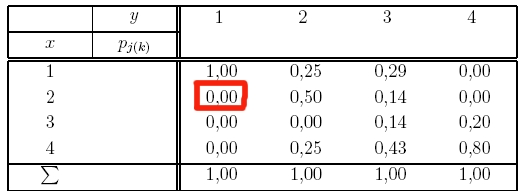
\includegraphics{b15.jpg}} 
\begin{tabular}{|cc||cccc|}
\hline
\multicolumn{1}{|c|}{\parbox{1.2cm}{\mbox{}}}& \parbox{1.2cm}{\mbox{}\hfill$y$\hfill\mbox{}} & \parbox{1.2cm}{\mbox{}\hfill 1 \hfill\mbox{}} & \parbox{1.2cm}{\mbox{}\hfill 2 \hfill\mbox{}} & \parbox{1.2cm}{\mbox{}\hfill 3 \hfill\mbox{}} & \parbox{1.2cm}{\mbox{}\hfill 4 \hfill\mbox{}}  \\[.75mm]
\cline{1-2}
\multicolumn{1}{|c|}{$x$} & $p_{j(k)}$ & & & &  \\[.75mm]
\hline\hline
1 & & 1,00 & 0,25 & 0,29 & 0,00 \\[.75mm]
2 & & \textcolor{red}{\bf 0,00} & 0,50 & 0,14 & 0,00 \\[.75mm]
3 & & 0,00 & 0,00 & 0,14 & 0,20 \\[.75mm]
4 & & 0,00 & 0,25 & 0,43 & 0,80 \\[.75mm]
\hline
$\sum$ & & 1,00 & 1,00 & 1,00 & 1,00 \\[.75mm]
\hline
\end{tabular}


\end{center}
\end{overprint}
}




\frame{\frametitle{Příklad 2}

Na plicním oddělení jisté nemocnice bylo náhodně vybráno 20 pacientů a zjišťovalo se u nich pohlaví (znak $X$: 0 -- muž, 1 -- žena) a kuřáctví (znak $Y$: 0 -- nekouří, 1 -- kouří). Výsledky:
\begin{center}
\small
\begin{tabular}{cccccccccc}
               (0,0)& (1,0)& (1,1)& (1,0) & (0,1)& (0,1)& (1,0)& (0,1)& (1,0)& (0,0)\\
               (1,0)& (0,1)& (0,1)& (1,0) & (1,0)& (1,1)& (0,0)& (0,0)& (1,0)& (1,1)\\
\end{tabular}
\normalsize
\end{center}
\begin{itemize}
\item[a)]	Sestrojte variační řady pro oba znaky
\begin{center}
\hspace*{-2cm}
\begin{tabular}{ccc}
Variační řada pro znak $X$&\hspace*{-1.8cm}&Variační řada pro znak $Y$\\[2mm]
\begin{tabular}{l|r|r|r|r}
&$n_j$&$p_j$&$N_j$&$F_j$\\ \hline
muž (0)&9&0,45&9&0,45\\
žena (1)&11&0,55&20&1,00\\
\end{tabular}
&&
\begin{tabular}{l|r|r|r|r}
&$n_j$&$p_j$&$N_j$&$F_j$\\ \hline
nekouří (0)&12&0,6&12&0,6\\
kouří (1)&8&0,4&20&1,0\\
\end{tabular}
\\
\end{tabular}
\end{center}
\end{itemize}
}


\frame{\frametitle{Příklad 2}
\begin{itemize}
\item[b)]	Sestrojte kontingenční tabulku absolutních četností pro oba znaky
\begin{center}
\begin{tabular}{l|cc|c} 
$X$ $\backslash$ $Y$&nekouří&kouří&$n_{i\cdot}$\\ \hline
muž&4&5&9\\ 
žena&8&3&11\\ \hline
$n_{\cdot j}$&12&8&20\\
\end{tabular}
\end{center}
\end{itemize}
}


\frame{\frametitle{Příklad 2}
\begin{itemize}
\item[c)]	Zjistěte procento mužů, žen, kuřáků, nekuřáků.
\begin{center}
	\begin{tabular}{l|l}
mužů je 45 \%&kuřáků je 40 \%\\
žen je 55 \%& nekuřáků je 60 \%\\[5mm]
\end{tabular}
\end{center}
\item[d)]	Kolik procent mužů kouří?\\
Mezi muži je 5/9 = 55,56 \% kuřáků. (z tabulky řádkově podmíněných četností)\\[5mm]
\item[e)]	Kolik procent kuřáků jsou muži?\\
Mezi kuřáky je 5/8 = 62,5 \% mužů. (z tabulky sloupcově podmíněných četností)
\end{itemize}
}


\frame{\frametitle{Příklad 2}
\begin{itemize}
\item[f)]	Sestrojte graf dvourozměrného rozložení četností.
\begin{center}
\scalebox{0.65}{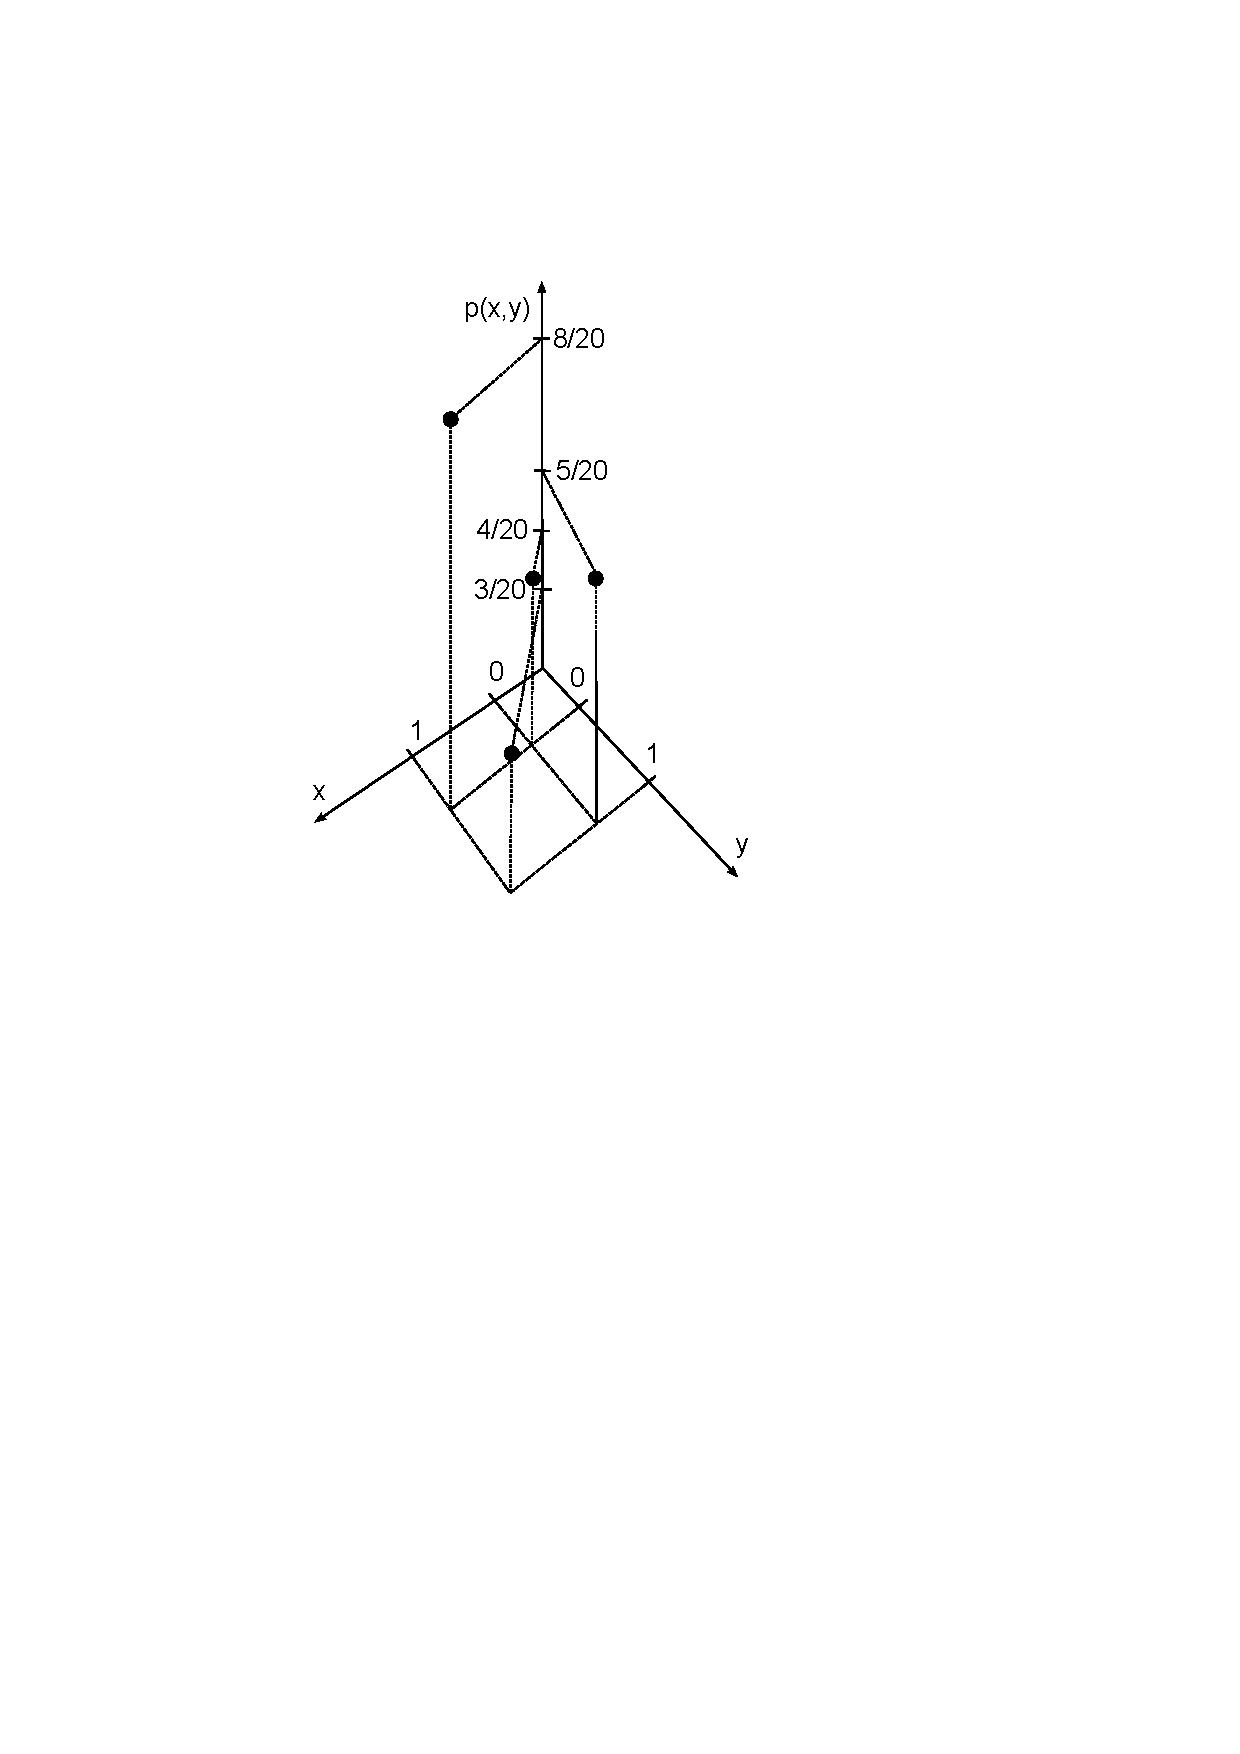
\includegraphics[viewport=150 415 360 710]{graf.pdf}}
\end{center}
\end{itemize}

}



\frame{
\centerline{\bf Intervalové rozdělení četností}
}



\frame {
  \frametitle{Intervalové rozdělení četnosti}
\begin{itemize}
\item  V některých datových souborech je počet variant znaku příliš veliký a použití
bodového rozdělení četností by vedlo k~nepřehledným a roztříštěným výsledkům.\\[1cm]

\item Nechť je dán jednorozměrný datový soubor. Jestliže počet variant znaku $X$
je blízký rozsahu souboru, pak přiřazujeme četnosti nikoliv jednotlivým variantám, ale celým intervalům hodnot. Hovoříme pak o {\bf intervalovém rozdělení četností}.
\end{itemize}
}

\frame {
  \frametitle{Stanovení třídících intervalů}
Číselnou osu rozložíme na intervaly typu $(-\infty, u_1], (u_1, u_2], \dots, (u_r, u_{r+1}],
(u_{r+1},\infty)$ tak, aby okrajové intervaly neobsahovaly žádnou pozorovanou hodnotu
znaku $X$. Užíváme označení
\begin{itemize}
\item $j$-tý třídicí interval znaku $X$, $j = 1, \dots, r$:
$$
(u_j, u_{j+1}],
$$
\item délka $j$-tého třídicího intervalu znaku $X$:
$$
d_j = u_{j+1} - u_j,
$$
\item střed $j$-tého třídicího intervalu znaku $X$:
$$
x_{[j]} =\frac{1}{2}(u_j + u_{j+1}).
$$
\end{itemize}
}

\frame {
  \frametitle{Stanovení třídících intervalů}
Třídicí intervaly volíme nejčastěji stejně dlouhé. Jejich počet určíme např.
pomocí {\bf Sturgesova pravidla}: 
$$
r = 1 + 3,3 \log v,
$$ 
kde $v$ je {\bf rozsah souboru}. 
}

\frame {
  \frametitle{Charakteristiky intervalových dat}
Nechť je dán jednorozměrný datový soubor rozsahu $n$. Hodnoty znaku $X$
roztřídíme do $r$ třídicích intervalů. Pro $j = 1, \dots, r$ definujeme:
\begin{itemize}
\item {\bf absolutní četnost} $j$-tého třídicího intervalu ve výběrovém souboru
$$
n_j = N(u_j < X \leq u_{j+1}),
$$
\item {\bf relativní četnost} $j$-tého třídicího intervalu ve výběrovém souboru
$$
p_j =\frac{n_j}{n},
$$
\item {\bf četnostní hustota} $j$-tého třídicího intervalu ve výběrovém souboru
$$
f_j =\frac{p_j}{d_j},
$$
\end{itemize}
}

\frame {
  \frametitle{Charakteristiky intervalových dat}
\begin{itemize}
\item {\bf absolutní kumulativní četnost} prvních $j$ třídicích intervalů ve výběrovém souboru
$$
N_j = N(X \leq u_{j+1}) = n_1 + \dots + n_j,
$$
\item {\bf relativní kumulativní četnost} prvních $j$ třídicích intervalů ve výběrovém souboru
$$
F_j =\frac{N_j}{n}= p_1 + \dots + p_j.
$$
\end{itemize}
}

\frame {
  \frametitle{Charakteristiky intervalových dat}
Tabulka typu
%\begin{center}\scalebox{0.5}{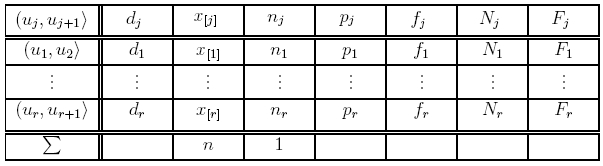
\includegraphics{i1.jpg}} \end{center}

\begin{center}
{\tabcolsep=3pt
\begin{tabular}{|c||c|c|c|c|c|c|c|}
\hline
\parbox[c][7mm]{1.7cm}{$(u_j, u_{j+1}\rangle$} & \parbox{1cm}{\mbox{}\hfill $d_j$ \hfill\mbox{}} & \parbox{1cm}{\mbox{}\hfill $x_{[j]}$ \hfill\mbox{}} & \parbox{1cm}{\mbox{}\hfill $n_j$ \hfill\mbox{}} & \parbox{1cm}{\mbox{}\hfill $p_j$ \hfill\mbox{}} & \parbox{1cm}{\mbox{}\hfill $f_j$ \hfill\mbox{}} & \parbox{1cm}{\mbox{}\hfill $N_j$ \hfill\mbox{}} & \parbox{1cm}{\mbox{}\hfill $F_j$ \hfill\mbox{}} \\[.75mm]
\hline\hline
\parbox[c][7mm]{1.7cm}{$(u_1,u_2\rangle$} & $d_1$ & $x_{[1]}$ & $n_1$ & $p_1$ & $f_1$ & $N_1$ & $F_1$ \\[.75mm]
\hline
$\vdots$ & $\vdots$ & $\vdots$ & $\vdots$ & $\vdots$ & $\vdots$ & $\vdots$ & $\vdots$ \\[.75mm]
\hline
\parbox[c][7mm]{1.7cm}{$(u_r,u_{r+1}\rangle$} & $d_r$ & $x_{[r]}$ & $n_r$ & $p_r$ & $f_r$ & $N_r$ & $F_r$ \\[2mm]
\hline\hline
$\sum$ & &  &$n$  & 1& & &\\[.75mm]
\hline
\end{tabular}}
\end{center}

se nazývá {\bf tabulka rozdělení četností}.
}



\frame {
  \frametitle{Histogram}

Intervalové rozdělení četností graficky znázorňujeme pomocí {\bf histogramu}.
Je to graf skládající se z $r$ obdélníků, sestrojených nad třídicími intervaly,
přičemž obsah $j$-tého obdélníku je roven relativní četnosti $p_j$ $j$-tého třídicího
intervalu, $j = 1, \dots, r$.\\[2mm] 
Histogram je shora omezen schodovitou čarou, která
je grafem funkce zvané {\bf hustota četnosti}
$$
f(x) = \left\{\begin{array}{ll} 
f_j& \mathsf{pro}\quad u_j < x \leq u_{j+1},\quad j = 1, \dots, r\\
0 &\mathsf{jinak.}\\
\end{array}\right.
$$
Pomocí hustoty četnosti zavedeme {\bf intervalovou empirickou distribuční funkci}
$$
F(x) =\int_{-\infty}^x f(t) dt.
$$
}
\frame {
  \frametitle{Vztah histogramu a empirické distribuční funkce}
\begin{center}\scalebox{0.4}{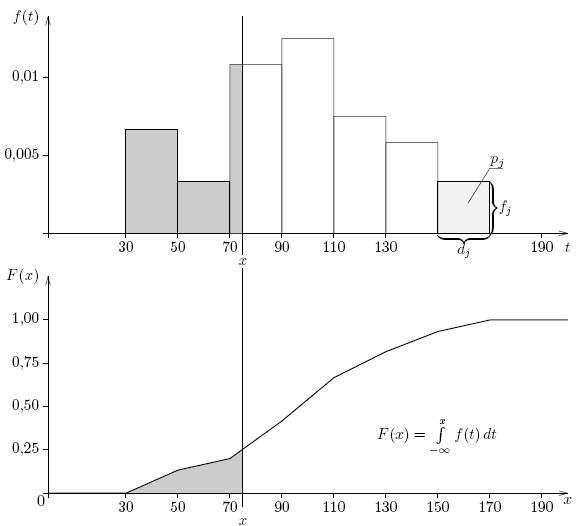
\includegraphics{hist.png}} \end{center}
}


\frame {
  \frametitle{Dvourozměrný soubor intervalových dat}

Nechť je dán dvourozměrný datový soubor
$$
\left[\begin{array}{cc}
x_1& y_1\\
\vdots&\vdots\\
x_n& y_n\\
\end{array}\right],
$$

kde hodnoty znaku $X$ roztřídíme do $r$ třídicích intervalů $(u_j, u_{j+1}]$, $j =1, \dots, r$ 
s délkami $d_1, \dots, d_r$ a hodnoty znaku $Y$ roztřídíme do $s$ třídicích
intervalů $(v_k, v_{k+1}]$, $k = 1, \dots, s$ s délkami $h_1, \dots, h_s$. Pak definujeme:
\begin{itemize}
\item {\bf simultánní absolutní četnost} $(j, k)$-tého třídicího intervalu:
$$
n_{jk} = N(u_j < X \leq u_{j+1} \wedge v_k < Y \leq v_{k+1}),
$$
\item {\bf simultánní relativní četnost} $(j, k)$-tého třídicího intervalu:
$$
p_{jk} =\frac{n_{jk}}{n},
$$
\end{itemize}
}


\frame {
  \frametitle{Dvourozměrný soubor intervalových dat}
\begin{itemize}
\item {\bf marginální absolutní četnost} $j$-tého třídicího intervalu pro znak $X$:
$$
n_{j.} = n_{j1} + \dots + n_{js},
$$
\item {\bf marginální relativní četnost} $j$-tého třídicího intervalu pro znak $X$:
$$
p_{j.} =\frac{n_{j.}}{n},
$$
\item {\bf marginální absolutní četnost} $k$-tého třídicího intervalu pro znak $Y$:
$$
n_{.k} = n_{1k} + \dots + n_{rk},
$$
\item {\bf marginální relativní četnost} $k$-tého třídicího intervalu pro znak $Y$:
$$
p_{.k} =\frac{n_{.k}}{n},
$$
\end{itemize}
}


\frame {
  \frametitle{Dvourozměrný soubor intervalových dat}
\begin{itemize}

\item {\bf simultánní četnostní hustota} v $(j, k)$-tém třídicím intervalu:
$$
f_{jk} =\frac{p_{jk}}{d_jh_k},
$$
\item {\bf marginální četnostní hustota} v $j$-tém třídicím intervalu pro znak $X$:
$$
f_{j.} =\frac{p_{j.}}{d_j},
$$
\item {\bf marginální četnostní hustota} v $k$-tém třídicím intervalu pro znak $Y$:
$$
f_{.k} =\frac{p_{.k}}{h_k}.
$$
\end{itemize}
}


\frame {
  \frametitle{Dvourozměrný datový soubor -- kontingenční tabulka}
Kteroukoliv ze simultánních četností zapisujeme do kontingenční tabulky.
Uveďme kontingenční tabulku simultánních absolutních četností:
\begin{center}

%\scalebox{0.5}{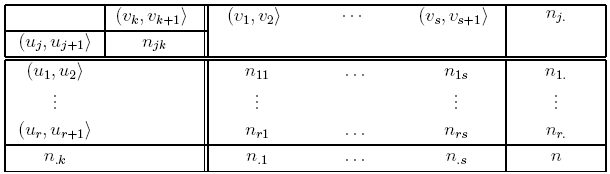
\includegraphics{i3.jpg}} 

\begin{tabular}{|cc||ccc|c|}
\hline
\multicolumn{1}{|c|}{\parbox{1.5cm}{\mbox{}}}& \parbox{1.5cm}{\mbox{}\hfill $(v_k,v_{k+1}\rangle$ \hfill\mbox{}} & \parbox{1.5cm}{\mbox{}\hfill $(v_1,v_2\rangle$ \hfill\mbox{}} & \parbox{1.1cm}{\mbox{}\hfill $\dots$ \hfill\mbox{}} & \parbox{1.5cm}{\mbox{}\hfill $(v_s,v_{s+1}\rangle$ \hfill\mbox{}} & \parbox{1.1cm}{\centering $n_{j.}$}\\[.75mm]
\cline{1-2}
\multicolumn{1}{|c|}{$(u_j,u_{j+1}\rangle$} & $n_{jk}$ & & & &  \\[.75mm]
\hline\hline
$(u_1,u_2\rangle$ & & $n_{11}$ & $\dots$ & $n_{1s}$ & $n_{1.}$ \\[.75mm]
$\vdots$ & & $\vdots$ & & $\vdots$ & $\vdots$ \\[.75mm]
$(u_r,u_{r+1}\rangle$ & & $n_{r1}$ & $\dots$ & $n_{rs}$ & $n_{r.}$ \\[.75mm]
\hline
$n_{.k}$ & & $n_{.1}$ & $\dots$ & $n_{.s}$ & $n$ \\[.75mm]
\hline
\end{tabular}

\end{center}
}

\frame {
  \frametitle{Simultánní hustota četnosti}
Funkce
$$
f(x, y) = \left\{ \begin{array}{ll}
f_{jk}& \mathsf{pro}\quad u_j < x \leq u_{j+1},\quad v_k < y \leq v_{k+1},\\
&j = 1, \dots, r,\quad k = 1,\dots, s\\
0 &\mathsf{jinak}\\
\end{array}\right.
$$
se nazývá simultánní {\bf hustota četnosti}.\\[2mm] 
Hustoty četnosti pro znaky $X$ a $Y$
(tzv. {\bf marginální hustoty četnosti}) odlišíme indexem takto:
$$
f_1(x) = \left\{ \begin{array}{ll}
 f_{j.}& \mathsf{pro}\quad u_j < x \leq u_{j+1},\quad j = 1, \dots, r\\
0& \mathsf{jinak}\\
\end{array}\right.
$$
$$
f_2(y) = \left\{ \begin{array}{ll} 
f_{.k}& \mathsf{pro}\quad v_k < y \leq v_{k+1},\quad k = 1, \dots, s\\
0 &\mathsf{jinak.}\\
\end{array}\right.
$$
}


\frame {
  \frametitle{Podmíněnné hustoty četnosti}

Funkce $f_{1\left|2\right. } \left(x\left|y\right. \right)$ zavedená vztahem $\forall x\in \mathbb R$:
$$
f_{1\left|2\right. } \left(x\left|y\right. \right)=\left\{
\begin{array}{ll} 
\frac{f\left(x,y\right)}{f_{2} \left(y\right)} &\mathrm{pro\; }f_{2} \left(y\right)>0 \\ 
0& \mathrm{jinak} 
\end{array}\right. 
$$ 
se nazývá \textbf{sloupcově podmíněná hustota četnosti.}\\[5mm]

Funkce $f_{2\left|1\right. } \left(y\left|x\right. \right)$ zavedená vztahem $\forall y\in \mathbb R$:
$$
f_{2\left|1\right. } \left(y\left|x\right. \right)=\left\{
\begin{array}{ll} 
\frac{f\left(x,y\right)}{f_{1} \left(x\right)}& \mathrm{pro\; }f_{1} \left(x\right)>0 \\ 
0 & \mathrm{jinak} 
\end{array}\right. 
$$ 
se nazývá \textbf{řádkově podmíněná hustota četnosti.}

}

\frame {
  \frametitle{Četnostní nezávislost}
Řekneme, že znaky $X$, $Y$ jsou v~daném výběrovém souboru \textbf{četnostně nezávislé} při intervalovém rozložení četností, jestliže 
$$
\forall j=1,\dots, r,\ \forall k=1,\dots, s: \quad f_{jk}=f_{j.}\cdot f_{.k}
$$ 
neboli 
$$
\forall (x,y)\in\mathbb R^2: f(x,y)=f_1(x)f_2(y).
$$
}

\frame {
  \frametitle{Četnostní nezávislost -- ekvivalentní definice}
Znaky $X$, $Y$ jsou v~daném výběrovém souboru \textbf{četnostně nezávislé} při intervalovém rozložení četností, jestliže platí: 
$$
\forall y\in \mathbb R,\ f_{2} \left(y\right)>0:\quad f_{1\left|2\right. } \left(x\left|y\right. \right)=f_{1} \left(x\right)
$$ 
resp. 
$$
\forall x\in \mathbb R,\ f_{1} \left(x\right)>0:\quad f_{2\left|1\right. } \left(y\left|x\right. \right)=f_{2} \left(y\right).
$$ 
}




\frame {
  \frametitle{Dvourozměrný datový soubor -- příklad}
U 50 náhodně vybraných srovnatelných firem byly zjišťovány náklady na reklamu v tisících Kč (znak $X$) a hrubý zisk opět v~tisících Kč (znak $Y$).
$$
\left[
\begin{array}{cc}
58 &178\\
68 &173\\
56 &170\\
60 &170\\
61 &173\\
71 &181\\
85 &184\\
80 &170\\
52 &172\\
72 &182\\
\end{array}\right]
\left[
\begin{array}{cc}
65 &170\\
57 &169\\
65 &169\\
60 &170\\
54 &162\\
52 &169\\
83 &182\\
60 &168\\
68 &173\\
63 &171\\
\end{array}\right]
\left[
\begin{array}{cc}
72 &177\\
90 &192\\
57 &176\\
51 &168\\
81 &190\\
73 &177\\
75 &179\\
71 &180\\
66 &178\\
67 &182\\
\end{array}\right]
\left[
\begin{array}{cc}
72 &191\\
57 &174\\
57 &160\\
56 &170\\
56 &172\\
52 &165\\
72 &185\\
75 &170\\
52 &163\\
63 &184\\
\end{array}\right]
\left[
\begin{array}{cc}
63 &172\\
58 &163\\
64 &174\\
52 &168\\
55 &164\\
67 &173\\
60 &170\\
55 &160\\
62 &172\\
70 &171\\
\end{array}\right]
$$
}
\frame {
  \frametitle{Dvourozměrný datový soubor -- příklad}
  
  Pro znak X stanovte optimální počet třídicích intervalů podle
Sturgesova pravidla, sestavte tabulku rozdělení četnosti, nakreslete
histogram a graf intervalové empirické distribuční funkce.\\[0.5cm]
\begin{overprint}
\onslide<1> Optimální počet třídicích intervalů je 7. Tabulka rozdělení četností:
\begin{center}

%\scalebox{0.5}{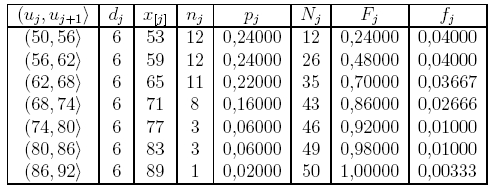
\includegraphics{i4.jpg}} 

\begin{tabular}{|c|c|c|c|c|c|c|c|}
 \hline $(u_j,u_{j+1}\rangle$ & $d_j$ & $x_{[j]}$ & $n_j$ & $p_j$ & $N_j$ & $F_j$ & $f_j$ \\ \hline
 $(50,56\rangle$ & 6 & 53 & 12 & 0,24000 & 12 & 0,24000 & 0,04000 \\
 $(56,62\rangle$ & 6 & 59 & 12 & 0,24000 & 24 & 0,48000 & 0,04000 \\
 $(62,68\rangle$ & 6 & 65 & 11 & 0,22000 & 35 & 0,70000 & 0,03667 \\
 $(68,74\rangle$ & 6 & 71 & 8 & 0,16000 & 43 & 0,86000 & 0,02666 \\
 $(74,80\rangle$ & 6 & 77 & 3 & 0,06000 & 46 & 0,92000 & 0,01000 \\
 $(80,86\rangle$ & 6 & 83 & 3 & 0,06000 & 49 & 0,98000 & 0,01000 \\
 $(86,92\rangle$ & 6 & 89 & 1 & 0,02000 & 50 & 1,00000 & 0,00333 \\\hline
\end{tabular}


\end{center}
\onslide<2>Histogram:
\begin{center}\scalebox{0.5}{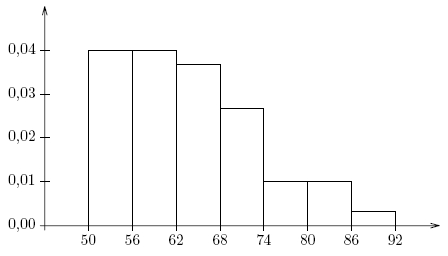
\includegraphics{i5.jpg}} \end{center}

\onslide<3>  Graf intervalové empirické distribuční funkce:
\begin{center}\scalebox{0.5}{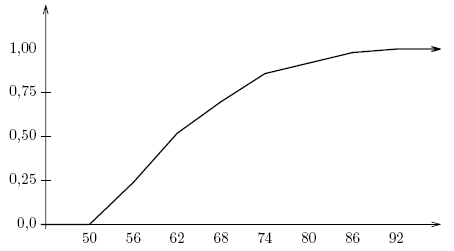
\includegraphics{i6.jpg}} \end{center}
\end{overprint}
}
\frame {
  \frametitle{Dvourozměrný datový soubor -- příklad}
  \begin{overprint}
Pro vektorový znak $(X, Y )$ sestavte kontingenční tabulku absolutních četností a nakreslete dvourozměrný tečkový diagram.\\[0.2cm]
\onslide<1> Optimální počet třídicích intervalů pro znak $Y$ je 7. Kontingenční tabulka absolutních četností
\begin{center}\scalebox{0.45}{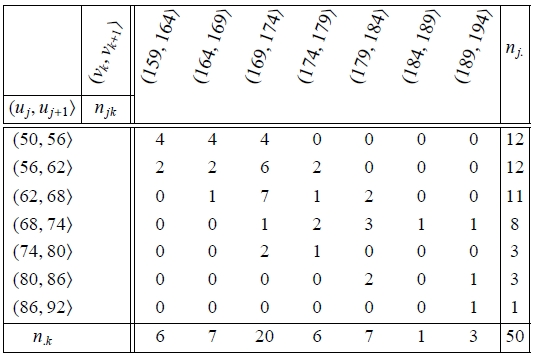
\includegraphics{i7.jpg}} \end{center}
\onslide<2>  Dvourozměrný tečkový diagram
\begin{center}\scalebox{0.5}{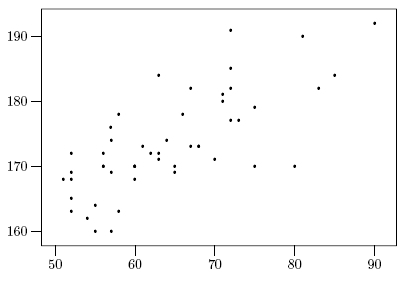
\includegraphics{i8.jpg}} \end{center}
\end{overprint}

}


\frame{
\centerline{\bf Číselné charakteristiky znaků}
}


\frame {
  \frametitle{Typy znaků}
  
Podle stupně kvantifikace znaky třídíme takto:\\[1cm]
\begin{itemize}
\item[(n)] {\bf Nominální znaky} připouštějí obsahovou interpretaci jedině relace rovnosti $x_1 = x_2$ (popřípadě $x_1 \neq x_2$), tj. hodnoty znaku představují jen číselné kódy kvalitativních pojmenování.\\[0.5cm] Např. městské tramvaje jsou očíslovány, ale např. č. 4 a 12 říkají jen to, že jde o různé tratě: nic jiného se z nich o vztahu obou tratí nedá vyčíst.\end{itemize}
}





\frame {
  \frametitle{Typy znaků}
  \begin{itemize}
\item[(o)] {\bf Ordinální znaky} připouštějí obsahovou interpretaci kromě relace rovnosti i v případě relace uspořádání $x_1 < x_2$ (popřípadě $x_1 > x_2$), tj. jejich uspořádání vyjadřuje větší nebo menší intenzitu zkoumané vlastnosti.\\[0.5cm] Např. školní klasifikace vyjadřuje menší nebo větší znalosti zkoušených (jedničkář je lepší než dvojkař), ale intervaly mezi známkami nemají obsahové interpretace (netvrdíme, že rozdíl ve znalostech mezi jedničkářem a dvojkařem je stejný jako mezi trojkařem a čtyřkařem. Podobný charakter mají různá bodování ve sportovních, uměleckých a jiných soutěžích.

\end{itemize}
}





\frame {
  \frametitle{Typy znaků}
  \begin{itemize}

\item[(i)] {\bf Intervalové znaky} připouštějí obsahovou interpretaci kromě relace rovnosti a uspořádání též u operace rozdílu $x_1 - x_2$ (popřípadě součtu $x_1 + x_2$), tj. stejný interval mezi jednou dvojicí hodnot a jinou dvojicí hodnot vyjadřuje i stejný rozdíl v extenzitě zkoumané vlastnosti.\\[0.5cm] Např. teplota měřená ve stupních Celsia představuje intervalový znak. Naměříme-li ve čtyřech dnech polední teploty 0, 2, 4, 6, znamená to, že každým dnem stoupla teplota o 2 stupně Celsia. Bylo by však chybou interpretovat tyto údaje tvrzením, že ze druhého na třetí den vzrostla teplota dvakrát, kdežto ze třetího na čtvrtý pouze jedenapůlkrát.

\end{itemize}
}





\frame {
  \frametitle{Typy znaků}
  \begin{itemize}

\item[(p)] {\bf Poměrové znaky} umožňují obsahovou interpretaci kromě relace rovnosti a uspořádání a operace rozdílu ještě u operace podílu $x_1/x_2$ (popřípadě součinu $x_1\cdot x_2$), tj. stejný poměr mezi jednou dvojicí hodnot a druhou dvojicí hodnot znamená i stejný podíl v extenzitě zkoumané vlastnosti.\\[0.5cm] Např. má-li jedna osoba hmotnost 150 kg a druhá 75 kg, má smysl prohlásit, že první je dvakrát hmotnější než druhá.\\

\end{itemize}
}





\frame {
  \frametitle{Typy znaků}
  Zvláštní postavení mají:\\[1cm]
  \begin{itemize}


\item[(a)] {\bf Alternativní znaky}, které nabývají jen dvou hodnot, např. 0, 1, což znamená absenci a prezenci nějakého jevu.\\[0.5cm] Například 0 bude znamenat neúspěch, 1 úspěch při řešení určité úlohy. Alternativní znaky mohou být ztotožněny s kterýmkoliv z předcházejících typů.
\end{itemize}
}

\frame{ \frametitle{Charakteristiky polohy}
\begin{itemize}
\item
Pro nominální znaky používáme jako charakteristiku polohy {\bf modus}. U bodového rozdělení četností je to nejčetnější varianta znaku, u intervalového střed nejčetnějšího třídicího intervalu.
\item
Pro ordinální znaky používáme jako charakteristiku polohy $\alpha$-{\bf kvantil}. Jeli $\alpha \in (0,1)$, pak $\alpha$-kvantil $x_\alpha$ je číslo, které rozděluje uspořádaný datový soubor na dolní úsek, obsahující aspoň podíl $\alpha$ všech dat a na horní úsek obsahující aspoň podíl $1 - \alpha$ všech dat. Pro výpočet $\alpha$-kvantilu slouží algoritmus:
\begin{itemize}
\item $n\alpha$ je celé číslo $c$: $x_\alpha=\frac{x_{(c)}+x_{(c+1)}}{2} $
\item $n\alpha$ je necelé číslo: zaokrouhlíme nahoru na nejbližší celé číslo $c$ a $x_{\alpha}=x_{(c)}$.
\end{itemize}
Pro speciálně zvolená $\alpha$ užíváme názvů: $x_{0.50}$ -- medián, $x_{0.25}$ -- dolní kvartil, $x_{0.75}$ -- horní kvartil, $x_{0.1},\dots, x_{0.9}$ -- decily, $x_{0.01},\dots, x_{0.99}$ -- percentily. 

\end{itemize}
}

\frame{ \frametitle{Charakteristiky polohy}
\begin{itemize}


\item
Pro intervalové a poměrové znaky slouží jako charakteristika polohy aritmetický průměr
 $$
 m_x=\frac{1}{n}\sum_{i=1}^n x_i.
 $$
 Lze ho interpretovat jako těžiště jednorozměrného tečkového digramu.
\end{itemize}
}


\frame{ \frametitle{Charakteristiky polohy -- příklad}
Pro datový soubor "hodnocení finančního zdraví několika firem I. hodnotitelem" vypočtěte medián a oba kvartily.\\[1cm]
\begin{overprint}
\onslide<1>
  \begin{center}
\begin{tabular}{c}
I. hodnotitel\\ \hline
2 \\
1 \\
4  \\
1  \\
1  \\
4  \\
3  \\
3 \\
1  \\
1 \\
\end{tabular}
\begin{tabular}{c}
I. hodnotitel\\ \hline
4 \\
4 \\
2 \\
4 \\
2 \\
4 \\
1  \\
4  \\
4  \\
1  \\
\end{tabular}
\end{center}
\onslide<2>
\begin{center}
\tabcolsep=2pt
    \begin{tabular}{|l|c|c|c|c|c|c|c|c|c|c|c|c|c|c|c|c|c|c|c|c|}
      \hline
  \textbf{Hodnoty}&    \textbf{1} & \textbf{1} & \textbf{1} & \textbf{1} & \textbf{1} & \textbf{1} & \textbf{1} & \textbf{2} & \textbf{2} & \textbf{2} & \textbf{3} & \textbf{3} & \textbf{4} & \textbf{4} & \textbf{4} & \textbf{4} & \textbf{4} & \textbf{4} & \textbf{4} & \textbf{4} \\
      \hline \hline
 \textbf{Pořadí} &  \parbox[t]{0.3cm}{\centerline{1}} & \parbox[t]{0.3cm}{\centerline{2}} & \parbox[t]{0.3cm}{\centerline{3}} & \parbox[t]{0.3cm}{\centerline{4}} & \parbox[t]{0.3cm}{\centerline{5}} & \parbox[t]{0.3cm}{\centerline{6}} & \parbox[t]{0.3cm}{\centerline{7}} & \parbox[t]{0.3cm}{\centerline{8}} & \parbox[t]{0.3cm}{\centerline{9}} & \parbox[t]{0.3cm}{\centerline{10}} & \parbox[t]{0.3cm}{\centerline{11}} & \parbox[t]{0.3cm}{\centerline{12}} & \parbox[t]{0.3cm}{\centerline{13}} & \parbox[t]{0.3cm}{\centerline{14}} & \parbox[t]{0.3cm}{\centerline{15}} & \parbox[t]{0.3cm}{\centerline{16}} & \parbox[t]{0.3cm}{\centerline{17}} & \parbox[t]{0.3cm}{\centerline{18}} & \parbox[t]{0.3cm}{\centerline{19}} & \parbox[t]{0.3cm}{\centerline{20}} \\
      \hline
    \end{tabular}\end{center}
\onslide<3> %%%%%%%%%%%%%%%%%%%%%%%%%%%%%%%%%%%%%%%%%%%%%%%%%%%%%%%%%%%%%%%%%%%%%%%%%%%%%%%%%%%%%%%%%%%%
\begin{center}
\tabcolsep=2pt
    \begin{tabular}{|l|c|c|c|c|c|c|c|c|c|c|c|c|c|c|c|c|c|c|c|c|}
      \hline
  \textbf{Hodnoty}&    \textbf{1} & \textbf{1} & \textbf{1} & \textbf{1} & \textbf{\textcolor{blue}{1}} & \textbf{\textcolor{blue}{1}} & \textbf{1} & \textbf{2} & \textbf{2} & \textbf{2} & \textbf{3} & \textbf{3} & \textbf{4} & \textbf{4} & \textbf{4} & \textbf{4} & \textbf{4} & \textbf{4} & \textbf{4} & \textbf{4} \\
      \hline \hline
 \textbf{Pořadí} &  \parbox[t]{0.3cm}{\centerline{1}} & \parbox[t]{0.3cm}{\centerline{2}} & \parbox[t]{0.3cm}{\centerline{3}} & \parbox[t]{0.3cm}{\centerline{4}} & \parbox[t]{0.3cm}{\centerline{\textcolor{red}{5}}} & \parbox[t]{0.3cm}{\centerline{\textcolor{red}{6}}} & \parbox[t]{0.3cm}{\centerline{7}} & \parbox[t]{0.3cm}{\centerline{8}} & \parbox[t]{0.3cm}{\centerline{9}} & \parbox[t]{0.3cm}{\centerline{10}} & \parbox[t]{0.3cm}{\centerline{11}} & \parbox[t]{0.3cm}{\centerline{12}} & \parbox[t]{0.3cm}{\centerline{13}} & \parbox[t]{0.3cm}{\centerline{14}} & \parbox[t]{0.3cm}{\centerline{15}} & \parbox[t]{0.3cm}{\centerline{16}} & \parbox[t]{0.3cm}{\centerline{17}} & \parbox[t]{0.3cm}{\centerline{18}} & \parbox[t]{0.3cm}{\centerline{19}} & \parbox[t]{0.3cm}{\centerline{20}} \\
      \hline
    \end{tabular}\end{center}

\begin{center}
\begin{tabular}{ccccc}
$\alpha$&	$n\alpha$&	$c$&	&	$x_\alpha$\\[2mm] \hline
0.25&	$20\cdot 0.25 =5$	&\textcolor{red}{5}&	$\frac{(\textcolor{blue}{1}+\textcolor{blue}{1})}{2}$&1\\[2mm]
%0.50&	10&	10	&$\frac{(2+3)}{2}$&	2.5\\[2mm]
%0.75&	15&	15&	$\frac{(4+4)}{2}$&	4\\[4mm]
%0.36& 7.2& 8 & 2&2\\
\end{tabular}
\end{center}
\onslide<4> %%%%%%%%%%%%%%%%%%%%%%%%%%%%%%%%%%%%%%%%%%%%%%%%%%%%%%%%%%%%%%%%%%%%%%%%%%%%%%%%%%%%%%%%%%%%

\begin{center}
\tabcolsep=2pt
    \begin{tabular}{|l|c|c|c|c|c|c|c|c|c|c|c|c|c|c|c|c|c|c|c|c|}
      \hline
  \textbf{Hodnoty}&    \textbf{1} & \textbf{1} & \textbf{1} & \textbf{1} & \textbf{1} & \textbf{1} & \textbf{1} & \textbf{2} & \textbf{2} & \textbf{\textcolor{blue}{2}} & \textbf{\textcolor{blue}{3}} & \textbf{3} & \textbf{4} & \textbf{4} & \textbf{4} & \textbf{4} & \textbf{4} & \textbf{4} & \textbf{4} & \textbf{4} \\
      \hline \hline
 \textbf{Pořadí} &  \parbox[t]{0.3cm}{\centerline{1}} & \parbox[t]{0.3cm}{\centerline{2}} & \parbox[t]{0.3cm}{\centerline{3}} & \parbox[t]{0.3cm}{\centerline{4}} & \parbox[t]{0.3cm}{\centerline{5}} & \parbox[t]{0.3cm}{\centerline{6}} & \parbox[t]{0.3cm}{\centerline{7}} & \parbox[t]{0.3cm}{\centerline{8}} & \parbox[t]{0.3cm}{\centerline{9}} & \parbox[t]{0.3cm}{\centerline{\textcolor{red}{10}}} & \parbox[t]{0.3cm}{\centerline{\textcolor{red}{11}}} & \parbox[t]{0.3cm}{\centerline{12}} & \parbox[t]{0.3cm}{\centerline{13}} & \parbox[t]{0.3cm}{\centerline{14}} & \parbox[t]{0.3cm}{\centerline{15}} & \parbox[t]{0.3cm}{\centerline{16}} & \parbox[t]{0.3cm}{\centerline{17}} & \parbox[t]{0.3cm}{\centerline{18}} & \parbox[t]{0.3cm}{\centerline{19}} & \parbox[t]{0.3cm}{\centerline{20}} \\
      \hline
    \end{tabular}\end{center}

\begin{center}
\begin{tabular}{ccccc}
$\alpha$&	$n\alpha$&	$c$&	&	$x_\alpha$\\[2mm] \hline
%0.25&	5	&5&	$\frac{(1+1)}{2}$&1\\[2mm]
0.50&	$20\cdot 0.5 =10$&	\textcolor{red}{10}	&$\frac{(\textcolor{blue}{2}+\textcolor{blue}{3})}{2}$&	2.5\\[2mm]
%0.75&	15&	15&	$\frac{(4+4)}{2}$&	4\\[4mm]
%0.36& 7.2& 8 & 2&2\\
\end{tabular}
\end{center}
\onslide<5>  %%%%%%%%%%%%%%%%%%%%%%%%%%%%%%%%%%%%%%%%%%%%%%%%%%%%%%%%%%%%%%%%%%%%%%%%%%%%%%%%%%%%%%%%%%%%

\begin{center}
\tabcolsep=2pt
    \begin{tabular}{|l|c|c|c|c|c|c|c|c|c|c|c|c|c|c|c|c|c|c|c|c|}
      \hline
  \textbf{Hodnoty}&    \textbf{1} & \textbf{1} & \textbf{1} & \textbf{1} & \textbf{1} & \textbf{1} & \textbf{1} & \textbf{2} & \textbf{2} & \textbf{2} & \textbf{3} & \textbf{3} & \textbf{4} & \textbf{4} & \textbf{\textcolor{blue}{4}} & \textbf{\textcolor{blue}{4}} & \textbf{4} & \textbf{4} & \textbf{4} & \textbf{4} \\
      \hline \hline
 \textbf{Pořadí} &  \parbox[t]{0.3cm}{\centerline{1}} & \parbox[t]{0.3cm}{\centerline{2}} & \parbox[t]{0.3cm}{\centerline{3}} & \parbox[t]{0.3cm}{\centerline{4}} & \parbox[t]{0.3cm}{\centerline{5}} & \parbox[t]{0.3cm}{\centerline{6}} & \parbox[t]{0.3cm}{\centerline{7}} & \parbox[t]{0.3cm}{\centerline{8}} & \parbox[t]{0.3cm}{\centerline{9}} & \parbox[t]{0.3cm}{\centerline{10}} & \parbox[t]{0.3cm}{\centerline{11}} & \parbox[t]{0.3cm}{\centerline{12}} & \parbox[t]{0.3cm}{\centerline{13}} & \parbox[t]{0.3cm}{\centerline{14}} & \parbox[t]{0.3cm}{\centerline{\textcolor{red}{15}}} & \parbox[t]{0.3cm}{\centerline{\textcolor{red}{16}}} & \parbox[t]{0.3cm}{\centerline{17}} & \parbox[t]{0.3cm}{\centerline{18}} & \parbox[t]{0.3cm}{\centerline{19}} & \parbox[t]{0.3cm}{\centerline{20}} \\
      \hline
    \end{tabular}\end{center}

\begin{center}
\begin{tabular}{ccccc}
$\alpha$&	$n\alpha$&	$c$&	&	$x_\alpha$\\[2mm] \hline
%0.25&	5	&5&	$\frac{(1+1)}{2}$&1\\[2mm]
%0.50&	10&	10	&$\frac{(2+3)}{2}$&	2.5\\[2mm]
0.75&	$20\cdot 0.75 =15$&	\textcolor{red}{15}&	$\frac{(\textcolor{blue}{4}+\textcolor{blue}{4})}{2}$&	4\\[4mm]
%0.36& 7.2& 8 & 2&2\\
\end{tabular}
\end{center}
\onslide<6>  %%%%%%%%%%%%%%%%%%%%%%%%%%%%%%%%%%%%%%%%%%%%%%%%%%%%%%%%%%%%%%%%%%%%%%%%%%%%%%%%%%%%%%%%%%%%

\begin{center}
\tabcolsep=2pt
    \begin{tabular}{|l|c|c|c|c|c|c|c|c|c|c|c|c|c|c|c|c|c|c|c|c|}
      \hline
  \textbf{Hodnoty}&    \textbf{1} & \textbf{1} & \textbf{1} & \textbf{1} & \textbf{1} & \textbf{1} & \textbf{1} & \textbf{\textcolor{blue}{2}} & \textbf{2} & \textbf{2} & \textbf{3} & \textbf{3} & \textbf{4} & \textbf{4} & \textbf{4} & \textbf{4} & \textbf{4} & \textbf{4} & \textbf{4} & \textbf{4} \\
      \hline \hline
 \textbf{Pořadí} &  \parbox[t]{0.3cm}{\centerline{1}} & \parbox[t]{0.3cm}{\centerline{2}} & \parbox[t]{0.3cm}{\centerline{3}} & \parbox[t]{0.3cm}{\centerline{4}} & \parbox[t]{0.3cm}{\centerline{5}} & \parbox[t]{0.3cm}{\centerline{6}} & \parbox[t]{0.3cm}{\centerline{7}} & \parbox[t]{0.3cm}{\centerline{\textcolor{red}{8}}} & \parbox[t]{0.3cm}{\centerline{9}} & \parbox[t]{0.3cm}{\centerline{10}} & \parbox[t]{0.3cm}{\centerline{11}} & \parbox[t]{0.3cm}{\centerline{12}} & \parbox[t]{0.3cm}{\centerline{13}} & \parbox[t]{0.3cm}{\centerline{14}} & \parbox[t]{0.3cm}{\centerline{15}} & \parbox[t]{0.3cm}{\centerline{16}} & \parbox[t]{0.3cm}{\centerline{17}} & \parbox[t]{0.3cm}{\centerline{18}} & \parbox[t]{0.3cm}{\centerline{19}} & \parbox[t]{0.3cm}{\centerline{20}} \\
      \hline
    \end{tabular}\end{center}

\begin{center}
\begin{tabular}{ccccc}
$\alpha$&	$n\alpha$&	$c$&	&	$x_\alpha$\\[2mm] \hline
%0.25&	5	&5&	$\frac{(1+1)}{2}$&1\\[2mm]
%0.50&	10&	10	&$\frac{(2+3)}{2}$&	2.5\\[2mm]
%0.75&	15&	15&	$\frac{(4+4)}{2}$&	4\\[4mm]
0.36& $20\cdot 0.36 =7.2$& \textcolor{red}{8} & \textcolor{blue}{2}&2\\
\end{tabular}
\end{center}
\onslide<7>  %%%%%%%%%%%%%%%%%%%%%%%%%%%%%%%%%%%%%%%%%%%%%%%%%%%%%%%%%%%%%%%%%%%%%%%%%%%%%%%%%%%%%%%%%%%%

\begin{center}
\tabcolsep=2pt
    \begin{tabular}{|l|c|c|c|c|c|c|c|c|c|c|c|c|c|c|c|c|c|c|c|c|}
      \hline
  \textbf{Hodnoty}&    \textbf{1} & \textbf{1} & \textbf{1} & \textbf{1} & \textbf{1} & \textbf{1} & \textbf{1} & \textbf{2} & \textbf{2} & \textbf{2} & \textbf{3} & \textbf{3} & \textbf{4} & \textbf{4} & \textbf{4} & \textbf{4} & \textbf{4} & \textbf{4} & \textbf{4} & \textbf{4} \\
      \hline \hline
 \textbf{Pořadí} &  \parbox[t]{0.3cm}{\centerline{1}} & \parbox[t]{0.3cm}{\centerline{2}} & \parbox[t]{0.3cm}{\centerline{3}} & \parbox[t]{0.3cm}{\centerline{4}} & \parbox[t]{0.3cm}{\centerline{5}} & \parbox[t]{0.3cm}{\centerline{6}} & \parbox[t]{0.3cm}{\centerline{7}} & \parbox[t]{0.3cm}{\centerline{8}} & \parbox[t]{0.3cm}{\centerline{9}} & \parbox[t]{0.3cm}{\centerline{10}} & \parbox[t]{0.3cm}{\centerline{11}} & \parbox[t]{0.3cm}{\centerline{12}} & \parbox[t]{0.3cm}{\centerline{13}} & \parbox[t]{0.3cm}{\centerline{14}} & \parbox[t]{0.3cm}{\centerline{15}} & \parbox[t]{0.3cm}{\centerline{16}} & \parbox[t]{0.3cm}{\centerline{17}} & \parbox[t]{0.3cm}{\centerline{18}} & \parbox[t]{0.3cm}{\centerline{19}} & \parbox[t]{0.3cm}{\centerline{20}} \\
      \hline
    \end{tabular}\end{center}

\begin{center}
\begin{tabular}{ccccc}
$\alpha$&	$n\alpha$&	$c$&	&	$x_\alpha$\\[2mm] \hline
0.25&	$20\cdot 0.25 =5$	&5&	$\frac{(1+1)}{2}$&1\\[2mm]
0.50&	$20\cdot 0.5 =10$&	10	&$\frac{(2+3)}{2}$&	2.5\\[2mm]
0.75&	$20\cdot 0.75 =15$&	15&	$\frac{(4+4)}{2}$&	4\\[4mm]
0.36& $20\cdot 0.36 =7.2$& 8 & 2&2\\
\end{tabular}
\end{center}
\end{overprint}
}

\frame{\frametitle{Charakteristiky variability}
Jako charakteristika variability může sloužit {\bf kvartilová odchylka}
$$
IQR= x_{0.75}-x_{0.25}.
$$
Nejpoužívanější charakteristikou variability je však {\bf rozptyl}
 $$
 s^2_x=\frac{1}{n}\sum_{i=1}^n(x_i-m_x)^2
 $$
či {\bf směrodatná odchylka} $s_x = \sqrt{s_x^2}$. 
 
 }

\frame{\frametitle{Charakteristiky variability}
\begin{itemize}
\item Pomocí průměru a  směrodatné odchylky zavedeme {\bf standardizovanou
hodnotu} $\frac{x_i-m_x}{s_x}$ (vyjadřuje, o kolik směrodatných odchylek se $i$-tá hodnota odchýlila od průměru).
 \item
Rozptyl vychází v kvadrátech jednotek, v nichž byl měřen znak $X$, proto raději používáme směrodatnou odchylku $s$. 

\item
Pro poměrové znaky používáme jako charakteristiku variability {\bf koeficient
variace}  $\frac{s_x}{m_x}$. Je to bezrozměrné číslo, které se často vyjadřuje v procentech. Umožňuje porovnat variabilitu několika znaků. 

\item Jsou-li všechny hodnoty poměrového znaku kladné, pak jako charakteristiku polohy lze užít geometrický průměr $\sqrt[n]{x_1\cdot \dots \cdot x_n}$.
\end{itemize}
}



\frame{\frametitle{Dvourourozměrný datový soubor -- charakteristiky}
Pro dvourourozměrný datový soubor
$$
\left[
\begin{array}{cc}
x_1& y_1\\
\vdots&\vdots\\
x_n &y_n\\
\end{array}\right]
,
$$ 
kde znaky $X$ a $Y$ jsou intervalového či poměrového typu, používáme jako charakteristiku společné variability znaků $X$ a $Y$ kolem jejich průměrů \bf{kovarianci}
$$
s_{xy}=\frac{1}{n}\sum_{i=1}^n(x_i-m_x)(y_i-m_y).
$$
 %Kovariance je průměrem součinů centrovaných hodnot. Pokud se nadprůměrné (podprůměrné) hodnoty znaku X sdružují s nadprůměrnými (podprůměrnými) hodnotami znaku Y, budou součiny centrovaných hodnot Xi - mi a VÍ - ITT-2 vesměs kladné a jejich průměr (tj. kovariance) rovněž. Znamená to, že mezi znaky X, Y existuje určitý stupeň přímé lineární závislosti. Pokud se nadprůměrné (podprůměrné) hodnoty znaku X sdružují s podprůměrnými (nadprůměrnými) hodnotami znaku Y, budou součiny centrovaných hodnot vesměs záporné a jejich průměr rovněž. Znamená to, že mezi znaky X a Y existuje určitý stupeň nepřímé lineární závislosti. Je-li kovariance nulová, pak řekneme, že znaky X, Y jsou nekorelované a znamená to, že mezi nimi neexistuje žádná lineární závislost.
 }
 \frame{\frametitle{Dvourourozměrný datový soubor -- charakteristiky}
Jsou-li směrodatné odchylky $s_x$, $s_y$ nenulové, pak definujeme {\bf koeficient korelace} znaků $X$, $Y$ vzorcem
 $$
 r_{xy}=\frac{s_{xy}}{s_xs_y}.
 $$
 
Pro koeficient korelace platí $- 1 \leq r_{xy} \leq 1$ a rovnosti je dosaženo právě když mezi hodnotami $x_1,\dots, x_n$ a $y_1,\dots, y_n$ existuje úplná lineární závislost, tj. existují konstanty $a$, $b$ tak, že $y_i = a + bx_i$, $i = 1,\dots ,n$, přičemž znaménko $+$ platí pro $b > 0$, znaménko $-$ pro $b < 0$.  
}



\frame{\frametitle{Dvourourozměrný datový soubor -- charakteristiky}

Představu o významu
hodnot koeficientu korelace podávají následující dvourozměrné tečkové diagramy.
 \begin{center}
 \scalebox{0.5}{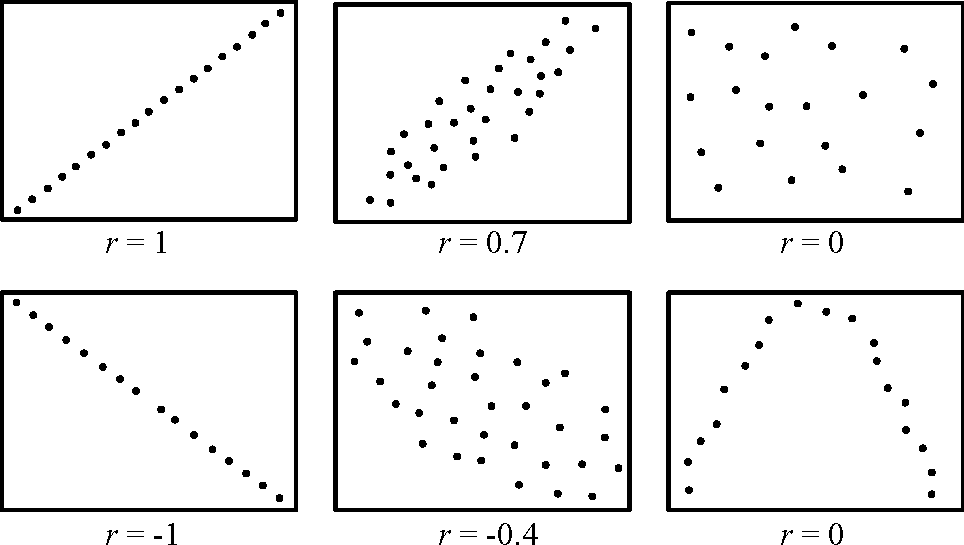
\includegraphics{korelace_new.pdf}}
\end{center}
}


\frame{\frametitle{Vážené číselné charakteristiky}
\begin{itemize}
	\item Vážený aritmetický průměr
$$
m=\frac{1}{n}\sum_{j=1}^rn_jx_{[j]}
$$
	\item Vážený rozptyl
$$
s^2=\frac{1}{n}\sum_{j=1}^rn_j(x_{[j]}-m)^2
$$
	\item Vážená kovariance
$$
s_{12}=\frac{1}{n}\sum_{j=1}^r\sum_{k=1}^rn_{jk}(x_{[j]}-m_1)(y_{[k]}-m_2)
$$
\end{itemize}

  
}

\frame{\frametitle{Vážené číselné charakteristiky - použití}
Mějme data zadaná následujícím způsobem:
$$
\begin{tabular}{|l|c|c|c|}
\hline
Výše dotace (v milionech) & 1 & 2 & 5\\ \hline
Počet & 4& 3&1\\ \hline
\end{tabular}
$$
\begin{itemize}
	\item Hodnot je celkem 8, nikoliv 3 (častá chyba).
	\item Pokud máme spočítat průměr, můžeme to provést obvyklým způsobem:
$$
m=\frac{1 + 1+ 1+1+2+2+2+5}{8},
$$
	\item anebo úsporněji podle vzorce pro vážený průměr:
$$
m=\frac{4\cdot1 + 3\cdot2+1\cdot5}{8}.
$$\end{itemize}

  
}


\frame{\centerline{\bf Regresní přímka}}


\frame{\frametitle{Regresní přímka}

\begin{itemize}
\item
Cílem regresní analýzy je vystižení závislosti hodnot znaku $Y$ na hodnotách znaku $X$. Při tom je nutné vyřešit dva problémy: \\[3mm]
\begin{itemize}
\item jaký typ funkce použít k vystižení dané závislosti a \\[3mm]
\item jak stanovit konkrétní parametry zvoleného typu funkce?\\[5mm]
\end{itemize} 
\item Typ funkce určíme buď logickým rozborem zkoumané závislosti nebo se ho snažíme odhadnout pomocí dvourozměrného tečkového diagramu. 
\end{itemize}

}

\frame{\frametitle{Regresní přímka}

Zde se omezíme na lineární závislost $y = \beta_0 + \beta_1 x$. Odhady $b_0$ a $b_1$ neznámých parametrů $\beta_0$, $\beta_1$ získáme na základě dvourozměrného datového souboru metodou nejmenších čtverců. Požadujeme, aby průměr součtu čtverců odchylek skutečných a odhadnutých hodnot byl minimální, tj. aby výraz
 $$
 \frac{1}{n}\sum_{i=1}^n(y_i-\beta_0-\beta_1x_i)^2
 $$
nabýval svého minima vzhledem k $\beta_0$ a $\beta_1$. Tento výraz je minimální, jsou-li jeho první derivace podle $\beta_0$ a $\beta_1$ nulové. Stačí tyto derivace spočítat, položit je rovny 0 a řešit systém dvou rovnic o dvou neznámých, tzv. systém normálních rovnic.
 

 
}

\frame{\frametitle{Regresní přímka} 

Nechť je dán dvourozměrný datový soubor
a přímka $y = \beta_0 + \beta_1x$. Výraz
  $$
 C=\frac{1}{n}\sum_{i=1}^n(y_i-\beta_0-\beta_1x_i)^2
 $$
se nazývá rozptyl hodnot znaku $Y$ kolem přímky $y = \beta_0 + \beta_1x$. Přímka $y = b_0 + b_1x$, jejíž parametry minimalizují rozptyl $$y = \beta_0 + \beta_1x$$ v celém dvourozměrném prostoru, se nazývá {\bf regresní přímka} znaku $Y$ na znak $X$. 
}

\frame{\frametitle{Regresní přímka} 
\begin{itemize}
\item {\bf Regresní odhad} $i$-té hodnoty znaku $Y$ značíme 
$$
\hat{y}_i = b_0 + b_1x_i,\quad i = 1,\dots, n.
$$ \\[1cm]

\item Kvadrát koeficientu korelace znaků $X$, $Y$ se nazývá {\bf index determinace} a značí se ID$^2$.\\[3mm] 
\begin{itemize}
\item Index determinace udává, jakou část variability hodnot znaku $Y$ vystihuje regresní přímka. \\[3mm]
\item Nabývá hodnot z intervalu $\langle 0,1\rangle$. \\[3mm]
\item Čím je bližší 1, tím lépe vystihuje regresní přímka závislost $Y$ na $X$.
\end{itemize}
\end{itemize}

}

\frame{\frametitle{Regresní přímka} 
Nechť $y = b_0 + b_1 x$ je regresní přímka znaku $Y$ na znak $X$. Pak použitím metody nejmenších čtverců dostaneme
 $$
 b_1=\frac{s_{xy}}{s_x^2},\quad b_0=m_y-\frac{s_{xy}}{s_x^2}m_x.
 $$
 \begin{itemize}
 \item Parametr $b_0$ udává velikost posunutí regresní přímky na svislé ose (tj. udává, jaký je regresní odhad hodnoty znaku $Y$, nabývá-li znak $X$ hodnoty 0). 
 \item Směrnice $b_1$ udává, o kolik jednotek se změní hodnota znaku $Y$, změní-li se hodnota znaku $X$ o jednotku.
 \item Jestliže je $b_1 > 0$, dochází s růstem $X$ k růstu $Y$ a hovoříme o přímé závislosti hodnot znaku $Y$ na hodnotách znaku $X$. 
 \item Je-li $b_1 < 0$, dochází s růstem $X$ k poklesu $Y$ a hovoříme o nepřímé závislosti hodnot znaku $Y$ na hodnotách znaku $X$.
 \end{itemize}
}

\frame{\frametitle{Regresní přímka -- příklad}
\centerline{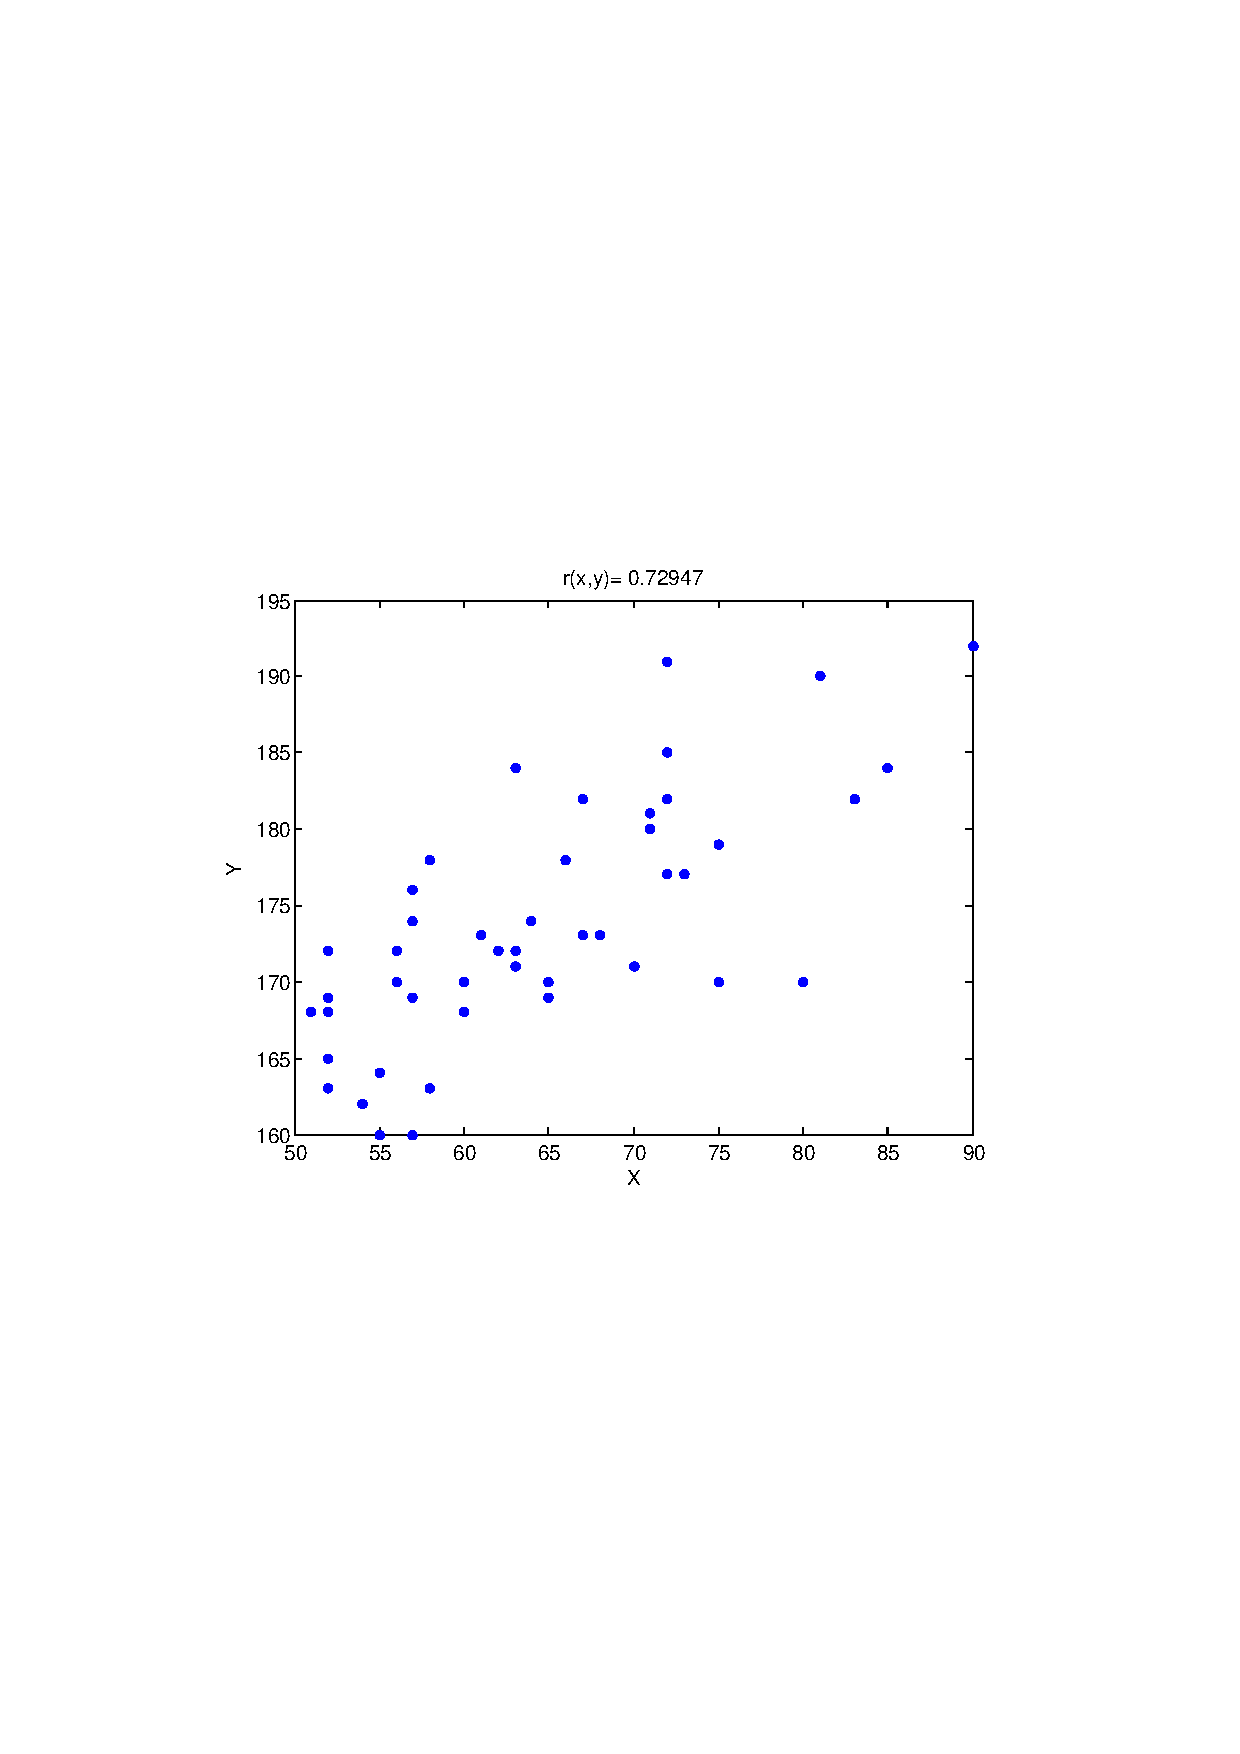
\includegraphics[bb= 60 80 540 570, scale=0.77]{reg1.pdf}}
}

\frame{\frametitle{Regresní přímka -- příklad}
\centerline{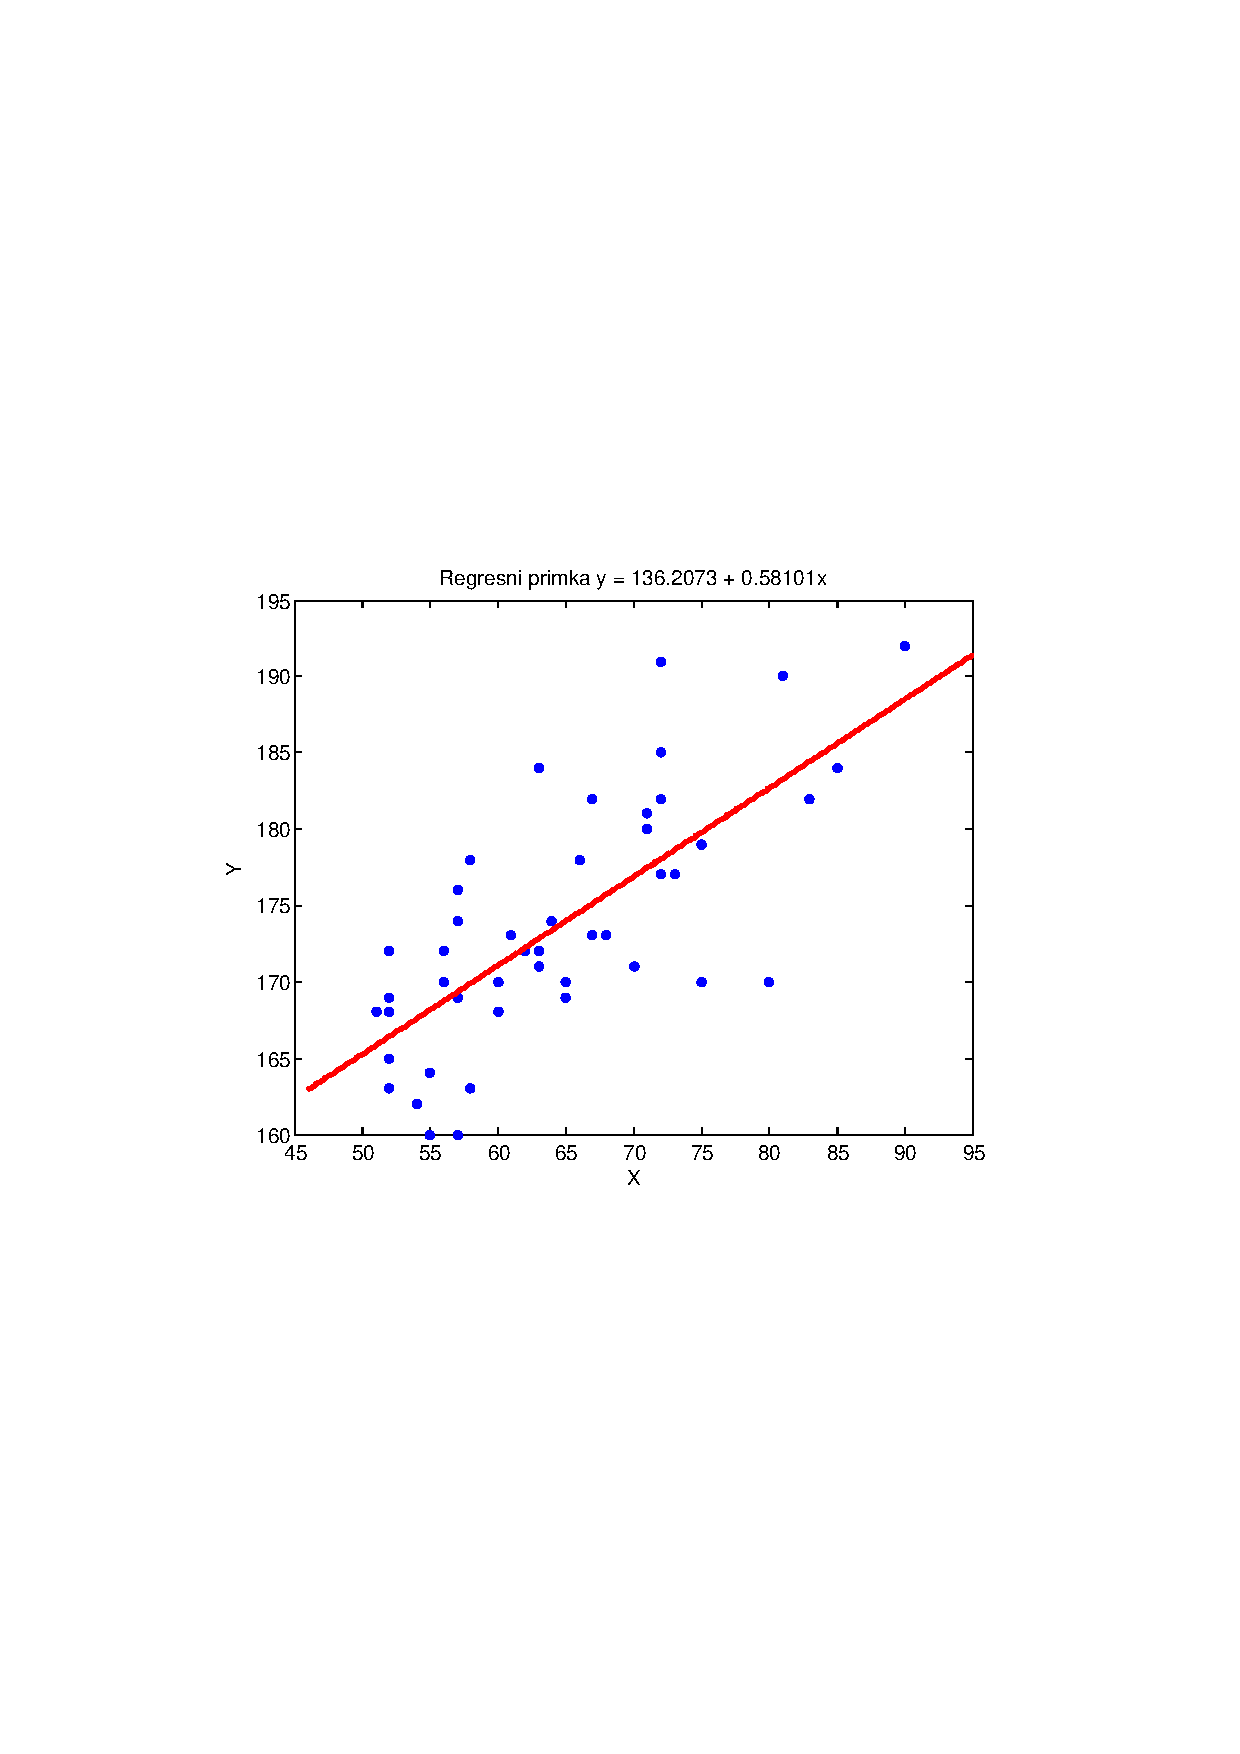
\includegraphics[bb= 60 80 540 570, scale=0.77]{reg2.pdf}}
}

\frame{\frametitle{Regresní přímka -- příklad}
\centerline{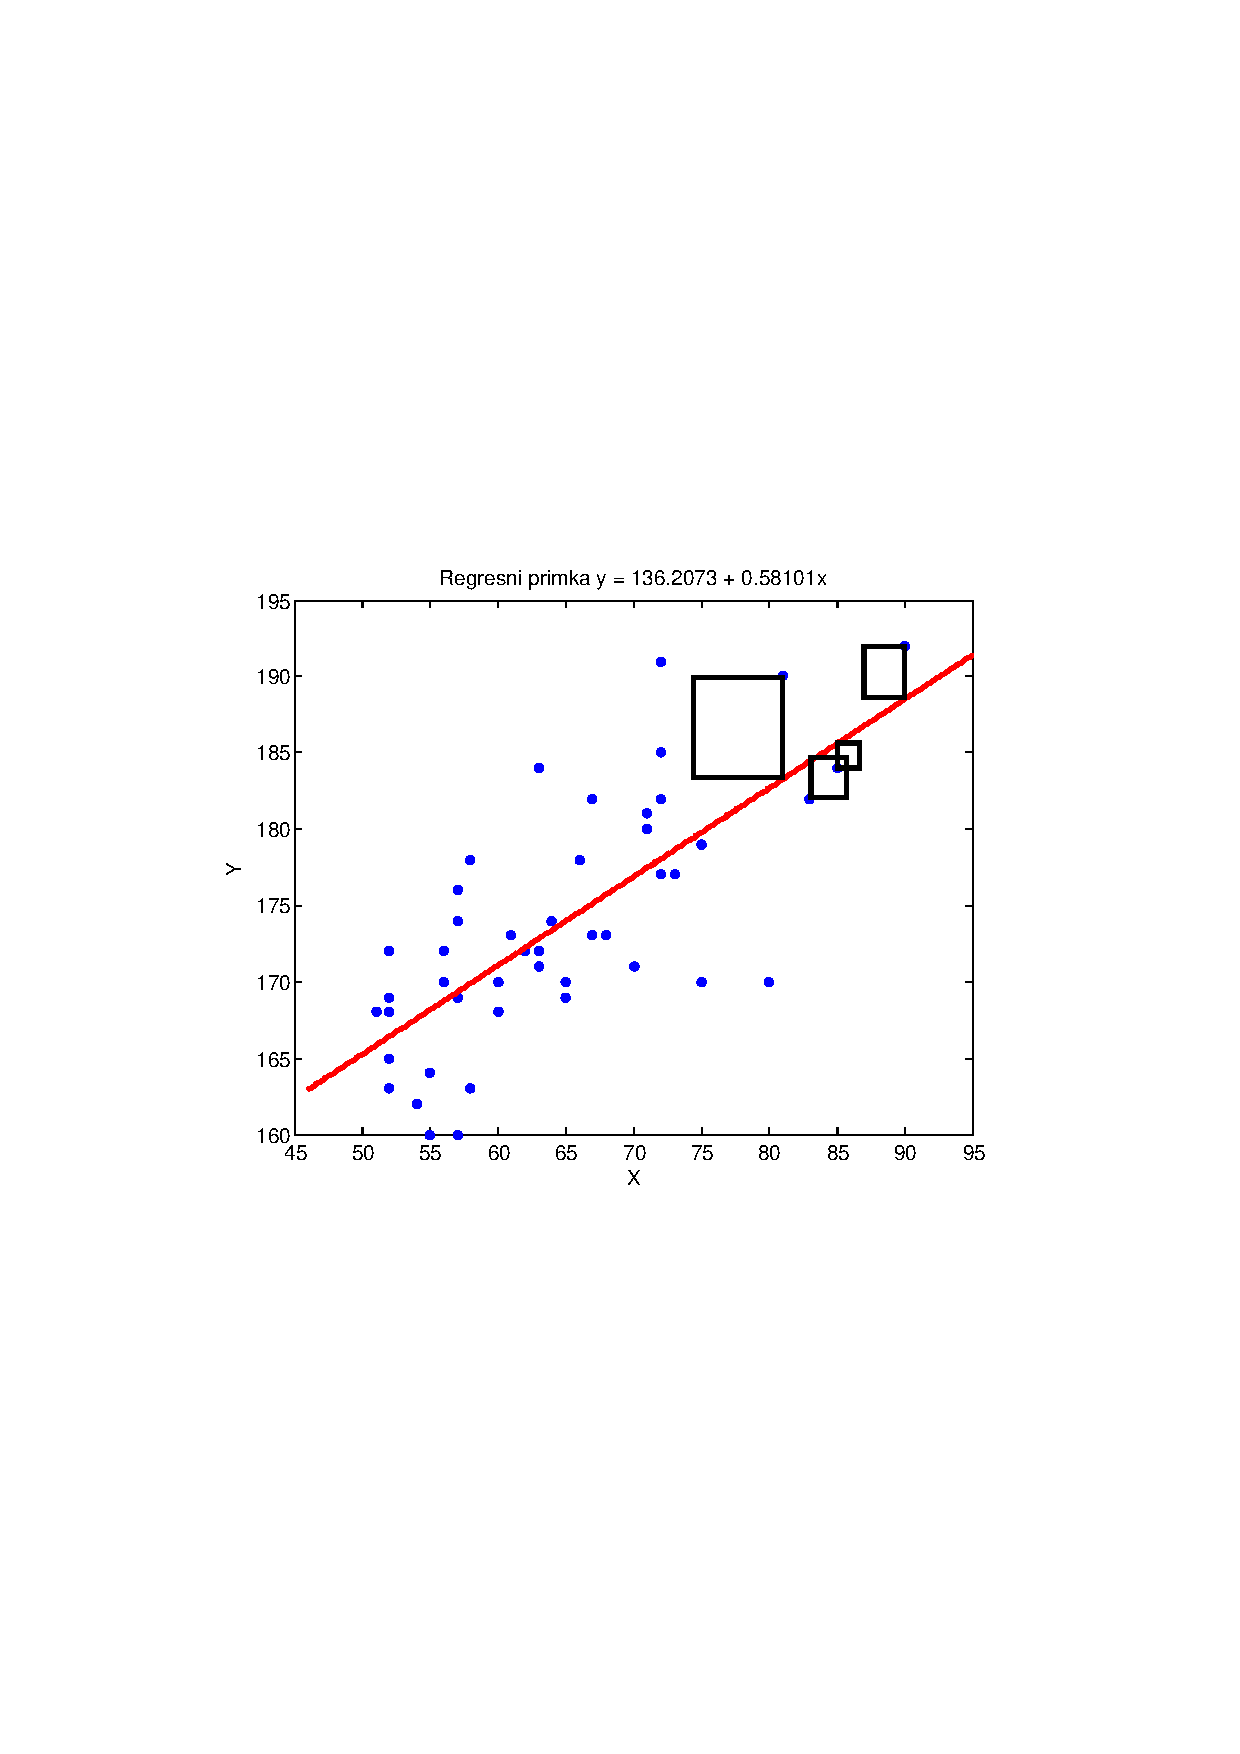
\includegraphics[bb= 60 80 540 570, scale=0.77]{reg3.pdf}}
}







\frame{
\centerline{\bf DĚKUJI ZA POZORNOST}}
\end{document}